\documentclass[11pt]{article}
\usepackage[margin=1in]{geometry}
\usepackage{amsmath,amssymb,graphicx,booktabs,xcolor,braket,hyperref}
\usepackage{placeins}   % \FloatBarrier keeps large floats inside their section
\usepackage{tikz}
\usepackage{quantikz}   % provides the quantikz environment (quantikz2)
\newcommand{\GCR}{\mathrm{GCR}}
\title{\textbf{Readout/Calibration of Erroneous GKP States}}
\author{Shraddha Singh}
\date{June 28, 2026}
\begin{document}
\maketitle

\noindent The Gaussian-Controlled-Rotation (GCR) of arXiv:2504.19992
suppresses the position-uncertainty error of an
oscillator-controlled qubit rotation by pairing each position-controlled kick with a compensating
momentum-controlled kick. Composed into the Abelian BB1 sequence, it promises a high-fidelity GKP
modular readout; here we ask whether that promise survives once the pulses must be physically
realizable and the hardware is noisy. The ideal performance for BB1(GCR) was shown through a non-unitary pulse which exactly cancelled the required errors due to Gaussianity. We show, first, that the approximation which this non-unitary pulse mimics cannot be reproduced by the unitary BB1(GCR) pulse, and GCR is the best any deterministic unitary achieves
at the no-error point (Sec.~\ref{sec:no-unitary-fix}). Nonetheless, the performance beating or matching GCR at all values of $\braket{x}$, be realized by the same pulse
\emph{probabilistically} via heralding (Sec.~\ref{sec:flagged}): we herald the three BB1 correction
pulses, leave the target a deterministic GCR, and post-select on the heralds, so that the
$\sim\!17\%$ of shots that pass carry the full ideal response yielding a readout infidelity of $5.7\times 10^{-4}$. Additionally, supporting our claim, a variationally optimized BB1(GCR)
alternative can yield the same performance, deterministically without any heralding or post-selection (Sec.~\ref{sec:qite-readout}): optimizing the correction amplitudes and axes over the
same short conditional-displacement ansatz reaches $1.5\times10^{-3}$, a factor $\sim\!5$ below bare
BB1, and then plateaus with added depth, so no short unitary matches the heralded floor---but the
coherent gain BB1(GCR) promises is real and physically achievable either way.

Neither route, however, survives contact with realistic noise. A failed herald ($\sim\!83\%$)
destroys the logical information through large back-action, and the unknown data state cannot be
re-prepared (Sec.~\ref{sec:endofline}); and once gate \emph{durations} are counted, both the
heralded and the compiled deterministic BB1(GCR) share the long $2\pi$ correction pulse that a
single GCR omits, so decoherence masks their coherent-floor advantage entirely and a single
GCR---an order of magnitude shorter, and just as accurate before noise---outperforms them both by
$\sim\!8\times$ once noise is included (Sec.~\ref{sec:qite-readout}), a verdict a full
master-equation simulation confirms (Sec.~\ref{sec:mesolve}). Two stress tests leave this ranking
intact: reading a codeword that idled under decay or dephasing before the read
(Sec.~\ref{sec:damage}), and reading one actively stabilized by noisy small-big-small rounds
(Sec.~\ref{sec:sbs}). BB1(GCR), whether heralded or deterministically compiled, thus emerges not as
an end-of-line readout but as a proof that the ideal correction is physically recoverable, and as
the tool of choice wherever post-selection or re-preparation is free, as in calibration and
known-state preparation (Sec.~\ref{sec:calibration}). Unless noted otherwise, all numbers are QuTiP
simulations at $\Delta=0.34$, $|\alpha|=\sqrt{\pi}/2$, and target angle $\theta_\mathrm{t}=\pi/2$,
with readout operating points at $\langle\hat x\rangle\in\sqrt{\pi}\,\mathbb{Z}$.

\section{Setup}
We build the readout by replacing each rotation of the Abelian BB1 sequence with a
Gaussian-Controlled-Rotation (GCR). We use the \emph{reversed} BB1 ordering, so that each
pre-correction acts on the state left by the preceding ideal rotation---the ordering the GCR
pre-correction structure requires,
\begin{equation}
\mathrm{BB1(GCR)}=
\GCR_{\phi_0}\!\Big(\tfrac{\theta_\mathrm{t}}{|\alpha|}\hat x\Big)\,
\GCR_{\phi_1}\!\Big(\tfrac{\pi}{|\alpha|}\hat x\Big)\,
\GCR_{3\phi_1}\!\Big(\tfrac{2\pi}{|\alpha|}\hat x\Big)\,
\GCR_{\phi_1}\!\Big(\tfrac{\pi}{|\alpha|}\hat x\Big),\qquad
\phi_1=\arccos\!\big(-\tfrac{\theta_\mathrm{t}}{4\pi}\big).
\label{eq:bb1gcr}
\end{equation}
whose four constituent rotation angles are $\{\pi,\,2\pi,\,\pi,\,\theta_\mathrm{t}\}$. Each GCR unit is a
position kick followed by a momentum pre-correction (its ``second pulse''),
\begin{equation}
\GCR_\phi\!\Big(\tfrac{\theta}{|\alpha|}\hat x\Big)
= \underbrace{e^{-i\frac{\theta}{2|\alpha|}\hat x\,\sigma_\phi}}_{\text{position kick}}\;
  \underbrace{e^{-i\frac{\theta\Delta^2}{2|\alpha|}\hat p\,\sigma_\gamma}}_{\text{pre-correction}},
\label{eq:gcrunit}
\end{equation}
whose pre-correction axis $\sigma_\gamma$ --- the second, momentum-controlled kick of each unit --- is
fixed by the ideal (error-free) qubit state $\ket{\zeta}$ reached after the preceding rotation, through
\begin{equation}
\sigma_\gamma\ket{\zeta}=i\,\sigma_\phi\ket{\zeta}.
\label{eq:axisrule}
\end{equation}
This condition is what lets the momentum kick undo, in the position basis, the Gaussian
position-uncertainty error of the next pulse, exactly as in the GCR construction. The task of the
composite pulse is to extract bitwise modular position information: a good readout produces a response
$P(+1)$ versus $\langle\hat x\rangle$ that approximates a square wave, reading $+1$ where
$\lfloor\langle\hat x\rangle/(2|\alpha|)\rfloor$ is even and $-1$ where it is odd. The whole question is
how faithfully the pre-correction \eqref{eq:gcrunit}--\eqref{eq:axisrule} can be built.

\section{The ideal readout is non-unitary}\label{sec:ideal}
Equation \eqref{eq:axisrule} is solved \emph{exactly}, as an operator, by the anti-Hermitian
choice $\sigma_\gamma\to i\sigma_\phi$. The pre-correction then becomes
\begin{equation}
e^{-i\frac{\theta\Delta^2}{2|\alpha|}\hat p\,(i\sigma_\phi)}
= e^{+\frac{\theta\Delta^2}{2|\alpha|}\hat p\,\sigma_\phi}\;\equiv\;M,
\label{eq:ideal}
\end{equation}
an ``imaginary conditional displacement'': a \emph{non-unitary} reweighting of the Gaussian along
$\hat x$ that cancels the position-uncertainty error at every angle, not just to leading order. Used
as the pre-correction of every GCR unit, it gives an almost perfect square wave (red dashed curve in
Fig.~\ref{fig:main}a), with operating-point error $P(-1)|_{x=0}\approx 4\times10^{-7}$. The catch is
that $i\sigma_\phi$ is anti-Hermitian, so $M$ is not a physical (unitary) gate.

\section{Why the physical (unitary) pulse fails --- and no unitary variant rescues it}\label{sec:no-unitary-fix}
A physical pre-correction must use a Hermitian axis, and this imposes two obstructions. The first is
\emph{realizability}: a Hermitian $\sigma_\gamma$ obeying \eqref{eq:axisrule} exists only when the qubit
is perpendicular to the pulse axis, $\braket{\zeta|\sigma_\phi|\zeta}=0$ (otherwise \eqref{eq:axisrule}
would equate a real number to an imaginary one), in which case $\sigma_\gamma=\hat n\times\hat\phi$ with
$\hat n$ the Bloch vector of $\ket{\zeta}$. BB1 does satisfy this at every step, since its $\pi$ and
$2\pi$ correction pulses shuttle the qubit between the poles $\pm\hat z$ and so keep it perpendicular to
the equatorial axes $\sigma_\phi$, deferring the sign-dependent readout rotation to the final target
pulse. The second obstruction is more serious: even where $\sigma_\gamma=\hat n\times\hat\phi$ exists,
the \emph{unitary} pre-correction reproduces the ideal $M$ only to leading order in the pulse angle
$\theta$. Because BB1's $2\pi$ pulse is four times the target angle, its higher-order residuals
dominate, and there the unitary correction does more harm than applying none at all: the readout washes
out entirely (Table~\ref{tab:cases}, Fig.~\ref{fig:main}a, green curve).

\begin{table}[h]
\centering
\begin{tabular}{lc}
\toprule
scheme (at $\langle x\rangle=0$) & $P(-1)$ \\
\midrule
ideal, non-unitary ($\sigma_\gamma=i\sigma_\phi$) & $4.1\times10^{-7}$ \\
bare BB1 (no GCR) & $6.1\times10^{-3}$ \\
physical (unitary) BB1(GCR) ($\sigma_\gamma=\hat n\times\hat\phi$) & $0.31$ \\
\bottomrule
\end{tabular}
\caption{Operating-point readout error. Only the non-unitary ideal beats bare; the physical
\emph{unitary} BB1(GCR) is washed out ($0.31$, i.e.\ essentially random, far worse than bare), and no
legal unitary variant (the whole sequence, or the $2\pi\to\pi+\pi$ split) does better.}
\label{tab:cases}
\end{table}

Nor can splitting the pulses rescue the deterministic readout. The readout peaks sit at
$x=2m|\alpha|$, where a pulse of angle-label $\eta$ rotates the qubit by $2\eta m$, so a BB1 correction
acts as an identity at every peak --- fixing one consistent, $x$-agnostic axis
$\sigma_\gamma=\hat n\times\hat\phi$ --- only for $\eta\in\pi\mathbb{Z}$. The only legal unitary
freedoms are therefore the whole sequence or the split $2\pi\to\pi+\pi$; the latter composes to
\emph{exactly} the same operator, while any sub-$\pi$ piece sends different peaks to different qubit
states and breaks the axis condition outright. Since a product of real conditional displacements can
never reproduce the non-unitary $i\sigma_\phi$ of \eqref{eq:ideal}, bare BB1 is the best any unitary
sequence achieves (Table~\ref{tab:cases}). The failure is \emph{structural} --- the unitary correction
is simply the wrong kind of operator --- and no tuning of sub-rotations or amplitudes can cure it.

\section{The flagged readout: a post-selected modular readout}\label{sec:flagged}
The only operator that beats bare is the non-unitary $M=e^{c\,\hat p\,\sigma_\phi}$ of
\eqref{eq:ideal} (with $c=\theta\Delta^2/2|\alpha|$), which cannot be a gate. It can be realized
\emph{probabilistically} by heralding, giving a \emph{post-selected} readout: the shots in which the
heralds succeed carry the full BB1(GCR) response. Heralding only the three \emph{corrections} (not the
target) both raises the success probability and keeps the outcome-defining pulse out of the
post-selection. This is the flagged readout, the practical payoff of this note.

\subsection{Construction}
BB1(GCR) has four pulses: three \emph{corrections} $\{\pi,2\pi,\pi\}$ and a final \emph{target}
$\{\pi/2\}$ whose measurement produces the $\pm1$ bit. We herald the ideal non-unitary $M$ on the
three correction pulses only (each with its own ancilla), and leave the target a \emph{deterministic}
(unitary) GCR. On the $\sim17\%$ of shots where all three heralds succeed, the corrections are the
exact $M$ and the whole sequence is the ideal BB1(GCR); \textbf{these are the shots we keep}.

This is genuine \emph{post-selection}, not a confidence tag on an otherwise-good bit. A failed herald
applies the complementary non-unitary Kraus operator, which corrupts the \emph{shared readout qubit}:
a failed shot then reads the \emph{wrong} bit ($P(-1)|_{x=0}=0.58$, worse than a coin flip), and
taking every shot regardless of the flag washes the readout out to $P(-1)|_{x=0}\approx0.26$ --- worse
than bare BB1. Failed shots must therefore be discarded. Leaving the \emph{target} deterministic (not
heralding it too) is what keeps the success probability at $\sim17\%$ rather than $\sim7\%$, and keeps
the bit-defining pulse out of the post-selection --- but it does \emph{not} make the readout
deterministic.

\subsection{The herald: block-encoding and gate sequence}\label{sec:herald-gates}
Heralding realizes $M$ by \emph{block-encoding}. Any $M$ with $\|M\|\le\lambda$ embeds in a unitary
$V$ on system$+$ancilla with $\langle0|V|0\rangle_{\mathrm{anc}}=M/\lambda$, so measuring the ancilla
and keeping $\ket0$ applies $M$ (up to normalization) with probability
\begin{equation}
P_{\mathrm{succ}}=\frac{\|M\ket{\psi}\|^2}{\lambda^2}.
\label{eq:psucc}
\end{equation}
The herald is a measurement of a \emph{separate ancilla}, not of the readout qubit: projecting the
readout qubit would delete the $\ket e$ branch that carries the answer, whereas $M$ must
\emph{reweight} the oscillator while keeping both qubit branches. Conditioning on the ancilla outcome
is exactly what ``apply $M$ and renormalize'' means in the simulation. For one correction pulse
(angle $\eta$, axis $\phi$, strength $c=\eta\Delta^2/2|\alpha|$) the elementary gadget
(Fig.~\ref{fig:circuit}) prepares a fresh ancilla $A$ in $\ket0$, applies
$W=\exp\!\big(-i\,c\,\hat p\,\sigma_\phi^{(S)}\otimes\sigma_y\big)$ --- the usual momentum-kick
conditional displacement (controlled by the system qubit through $\sigma_\phi$), now
\emph{additionally} controlled by $A$ through $\sigma_y$ --- and then applies a Hadamard to $A$ and
measures it, heralding success on $A=0$ and discarding $A=1$. Writing $\Theta=c\hat p\sigma_\phi$, the
$W$ step gives
$W\ket\psi\ket0=\cos\Theta\,\ket\psi\ket0+\sin\Theta\,\ket\psi\ket1$, and the Hadamard and measurement
project the $A=0$ branch onto $\tfrac1{\sqrt2}(\cos\Theta+\sin\Theta)\ket\psi$, while $A=1$ gives the
complementary $e^{-c\hat p\sigma_\phi}$.

\begin{figure}[h]
\centering
\begin{quantikz}[column sep=0.5cm,row sep=0.6cm]
\lstick{osc.} & \gate[2]{e^{-i\frac{\eta}{2|\alpha|}\hat x\sigma_\phi}} & \gate[3]{W=e^{-i c\,\hat p\,\sigma_\phi\otimes \sigma_y}} & \qw & \qw & \rstick{corrected} \\
\lstick{$\ket{\zeta}$ (sys.\ qubit)} &  &  & \qw & \qw & \qw \\
\lstick{$\ket{0}$ (ancilla $A$)} & \qw &  & \gate{H} & \meter{$0$?} & \rstick{herald}
\end{quantikz}
\caption{One heralded GCR correction (pulse angle $\eta$, axis $\phi$, strength
$c=\eta\Delta^2/2|\alpha|$). The position kick (first gate) is the ordinary conditional displacement
on oscillator$+$system qubit. The pre-correction is the \emph{ancilla-controlled} conditional
displacement $W=e^{-i c\,\hat p\,\sigma_\phi\otimes \sigma_y}$, followed by a Hadamard on the ancilla
and a measurement of the \emph{ancilla} (not the readout qubit). Outcome $\ket0$ heralds the
non-unitary correction $M/\lambda$; $\ket1$ is discarded.}
\label{fig:circuit}
\end{figure}

This elementary gadget reproduces $M$ only to \emph{first order} in $c$, since
$\cos\Theta+\sin\Theta\approx1+c\hat p\sigma_\phi\approx e^{c\hat p\sigma_\phi}$. Its success state overlaps the exact $M\ket\psi$ with a fidelity that tracks
the correction strength $c=\eta\Delta^2/2|\alpha|$: it is $0.996$ for the $\pi/2$ target ($c\approx0.10$)
and $0.94$ for the $\pi$ corrections ($c\approx0.20$), but only $0.47$ for the strong $2\pi$
correction ($c\approx0.41$). The $5.7\times10^{-4}$ readout
quoted below therefore assumes the \emph{exact} block-encoding of $M$ --- as realized in simulation
by applying $M$ and renormalizing, and physically by an exact block-encoding of $M$ on the low-energy
subspace (QSVT / qubitization) or by iterating the gadget. The single $W$+Hadamard step is the
leading-order intuition, not a faithful implementation of the $2\pi$ correction. $W$ itself compiles
from the echoed conditional-displacement primitive used for the two-mode gates: a
$\mathrm{CD}(c,\sigma_\phi)$ echoed by an ancilla $\pi$-pulse toggles the displacement sign with the
ancilla.

It is natural to ask whether amplitude amplification could remove the post-selection, since in quantum
algorithms one rarely discards the failure branch of a block-encoding: the linear-combination-of-unitaries (LCU)
construction is de-randomized by \emph{(oblivious) amplitude amplification}, which rotates the state
into the success branch with $O(\lambda)$ Grover-like reflections and \emph{no} measurement --- this
is why LCU-based Hamiltonian simulation is deterministic. That works, however, only when the encoded
target is (proportional to) a \emph{unitary}: then $\|M\ket\psi\|$ is input-independent and the
success/failure pair spans a fixed two-dimensional subspace the reflections close perfectly. Our
$M=e^{c\hat p\sigma_\phi}$ is a genuine \emph{contraction} --- it changes norm, which is the entire
source of its power --- so oblivious amplification does not apply: the success probability is bounded
by $\|M\ket\psi\|^2/\|\psi\|^2$ and can be pushed \emph{toward}, but never \emph{to}, unity. The
post-selection is therefore intrinsic, not an artifact of the elementary gadget. Put differently,
amplitude amplification de-randomizes exactly the block-encodings whose target could have been a gate
in the first place (unitary); $M$ can never join that class, which is the same non-unitarity that
made every deterministic attempt above fail.

\subsection{Why the target is left deterministic}
Heralding \emph{all four} pulses --- the target included --- reaches the ideal response
($4\times10^{-7}$) on its success branch (Table~\ref{tab:herald}), at $\sim7\%$ yield. Each herald
measures a correction's \emph{ancilla}, not the readout qubit, so the $g/e$ outcome is preserved: this
is a legitimate (if low-yield) heralded readout, not a post-selection on the bit. We nonetheless leave
the target a deterministic GCR, which raises the yield to $\sim17\%$ and uses one fewer ancilla, at
the cost of the target's own $\chi^4$ residual (a floor of $5.7\times10^{-4}$ rather than
$4\times10^{-7}$). Two corollaries follow: the target \emph{must} be a GCR --- a bare final rotation
gives $4.3\times10^{-2}$, worse than bare BB1 --- and the three corrections are best heralded as a
single block (splitting the $2\pi$ into $\pi+\pi$ gives the same operator, and post-selecting each
pulse separately only lowers the yield).

\begin{table}[h]
\centering
\begin{tabular}{lccccc}
\toprule
strength $s$ & 0 (bare) & 0.25 & 0.5 & 0.75 & 1.0 (ideal) \\
\midrule
$P(-1)|_{x=0}$ & $6.1\times10^{-3}$ & $2.5\times10^{-3}$ & $7.1\times10^{-4}$ & $6.6\times10^{-5}$ & $4.1\times10^{-7}$ \\
$P_{\mathrm{succ}}$ (global) & $1.0$ & $0.45$ & $0.13$ & $7.9\times10^{-3}$ & $1.7\times10^{-4}$ \\
$P_{\mathrm{succ}}$ (subspace $n\le40$) & $1.0$ & $0.62$ & $\mathbf{0.36}$ & $0.18$ & $\mathbf{0.071}$ \\
\bottomrule
\end{tabular}
\caption{\emph{Aside --- four-pulse heralding} (all four corrections heralded): success-branch readout
error and success probability vs correction strength $s$, for the naive global block-encoding and the
subspace-tailored one. The subspace bound reaches the ideal ($4\times10^{-7}$) at $\sim7\%$ yield, and
a tenfold improvement over bare at $\sim36\%$. Since the heralds act on ancillas (not the readout
qubit) this is a valid heralded readout; the three-herald readout of the main text is preferred for
its higher yield ($\sim17\%$). Not plotted.}
\label{tab:herald}
\end{table}

The yield is set by the subspace bound. The naive $\lambda=\|M\|$ over the whole truncated space
is wasteful, because $i\sigma_\phi$ amplifies the \emph{unpopulated} high-momentum tail. Restricting
the block-encoding to the low-energy input subspace ($n\le 40$ photons, containing $99.998\%$ of the
physical input) gives a far smaller $\lambda$ and hence a much higher yield --- this is what raises
the three-herald success from a few percent to $\sim17\%$.

\subsection{Results}
On its heralded branch the readout is a correct square wave at every peak (Fig.~\ref{fig:main}a),
with operating-point error $P(-1)|_{x=0}\approx5.7\times10^{-4}$ at herald success $\approx17\%$; the
remaining $\sim83\%$ are discarded (Sec.~\ref{sec:endofline}). This floor is set by the
\emph{un-heralded} target GCR's own $\chi^4$ residual, not the full ideal $4\times10^{-7}$; the three
corrections are otherwise exact. Two comparisons matter, and both use the deterministic
finite-energy single-GCR readout as the benchmark.

On the readout error itself (Fig.~\ref{fig:main}b), the heralding buys \emph{nothing} at a peak: a
single deterministic GCR already reaches $5.7\times10^{-4}$ there --- both are floored by the same
target-GCR residual --- and the two curves meet. What the post-selection earns instead is
\emph{robustness across the correctable region}. As one approaches the neighbouring peak, where the
correct bit flips to $-1$ so that $P(+1)$ is now the error, the heralded BB1(GCR) response stays
sharpest, driving $P(+1)$ down to $\approx5\times10^{-3}$ just off the peak against
$\approx5\times10^{-2}$ for the single GCR, which rolls off soonest (the unphysical ideal reaches
$\sim4\times10^{-7}$). This peak-location robustness --- BB1's defining role --- is the sole
readout-error advantage the post-selection wins over a deterministic GCR.

The back-action tells a similar story (Fig.~\ref{fig:main}c). On the success branch the readout is
nearly QND: the oscillator returns to the input at infidelity $\approx4\times10^{-3}$ across the whole
correctable region, whereas bare BB1 mangles an off-peak state, its infidelity peaking at
$\approx0.12$ at the bit-flip boundary. This gentleness is again shared with the single GCR
($\approx4\times10^{-3}$) --- a virtue of the GCR correction rather than of BB1(GCR) specifically ---
while the unphysical ideal is gentlest of all ($\approx6\times10^{-7}$, essentially perfect QND).
Either way, the $17\%$ of good shots read the bit \emph{and} preserve the state.

\begin{figure}[h]
\centering
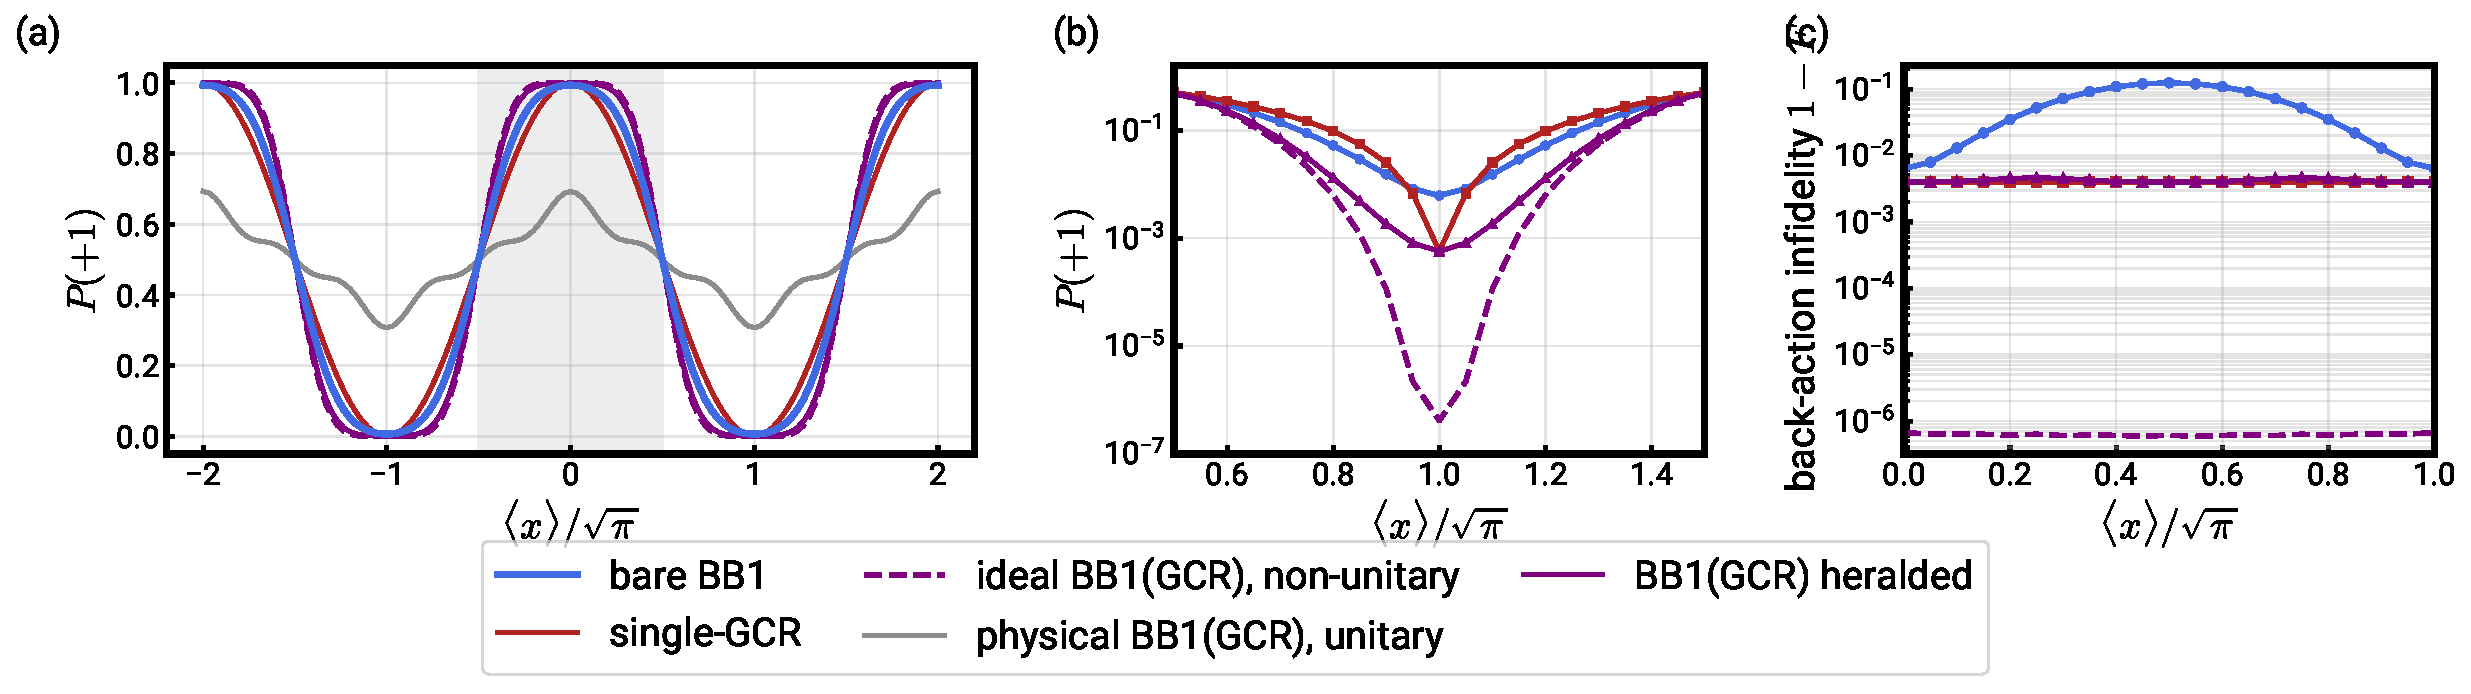
\includegraphics[width=\textwidth]{Supp_Figures/BB1_GCR_fixes.pdf}
\caption{\textbf{(a)} full-range readout $P(+1)$: bare BB1 (royalblue), single-GCR (firebrick), the
ideal non-unitary BB1(GCR) (purple dashed), the physically-realizable \emph{unitary} BB1(GCR) (grey;
$\sigma_\gamma=\hat n\times\hat\phi$, washes out to $\approx0.31$), and the heralded branch
(purple solid, the $\sim17\%$-herald branch: herald 3 corrections $+$ deterministic GCR target).
\textbf{(b)} $\log P(+1)$ zoomed near the neighbouring (odd) peak at $\langle x\rangle/\sqrt{\pi}{=}1$,
where the correct bit is $-1$ so $P(+1)$ \emph{is} the readout error: the ideal reaches
$\sim4\times10^{-7}$; among deployable curves heralded BB1(GCR) is sharpest ($\approx5\times10^{-3}$
just off the peak vs single-GCR's $\approx5\times10^{-2}$), the two meeting the common
$5.7\times10^{-4}$ target-GCR floor at the peak. \textbf{(c)} oscillator back-action infidelity $1-F$
(reduced-oscillator state vs the input) over $\langle x\rangle/\sqrt{\pi}\in[0,1]$ (log): the ideal
non-unitary BB1(GCR) is nearly perfectly QND ($\approx6\times10^{-7}$); single-GCR and heralded
stay $\approx4\times10^{-3}$; bare BB1 disturbs the state most, peaking at $\approx0.12$ at the
bit-flip boundary.}
\label{fig:main}
\end{figure}

\subsection{BB1(GCR) against all the readout schemes}\label{sec:context}
Figure~\ref{fig:readout} places BB1(GCR) alongside the other GKP readouts --- infinite-energy
(single CD), finite-energy GCR, Abelian BB1, the deployed GCR-BB1, and its two \emph{block} variants
(block~A, block~B) --- on the readout-error metric of the main text. The \emph{ideal} BB1(GCR) (the exact non-unitary correction) drives the error
\emph{below the Helstrom bound}, the fundamental limit on any \emph{deterministic} measurement. This
is not a contradiction: the ideal is a non-unitary limit, realized in the simulation only by the
per-pulse renormalization, and only a non-deterministic (post-selecting) scheme can beat Helstrom.

The catch is the herald success probability. To each non-unitary correction we attach the fraction
that the per-pulse $\texttt{.unit()}$ renormalization silently keeps,
$P_{\mathrm{succ}}=\|M\ket\psi\|^2/\lambda^2$, with $\lambda$ the largest singular value of the
correction over the populated low-energy subspace ($n\le40$). For the \emph{heralded} readout (herald
the three corrections, deterministic target) this is $\sim17\%$ (heralding the target too would reach
the ideal but at only $\sim7\%$). Because each herald acts on an ancilla, not the readout qubit, the
$g/e$ outcome is preserved --- but $\gtrsim83\%$ of shots are still discarded, which is why BB1(GCR)
is not a usable readout as it stands. But the prize is
plain: BB1(GCR) is, in principle, the \emph{best} readout available --- below every deterministic
scheme and even below Helstrom --- so if a route to a higher herald pass rate is found, BB1(GCR) is
the readout one should use. Panel~(b) is the mirror image for the \emph{logical-1} codeword: the same
readout error, now $P(g|\epsilon)=1-P(e|\epsilon)$, over the logical-1 peak. It dips to the same floors
at the logical-1 peak $\epsilon=\sqrt{\pi/2}$ (ideal $\sim10^{-10}$, heralded $\sim5.7\times10^{-4}$),
confirming the readout is symmetric between the two codewords.

\begin{figure}[h]
\centering
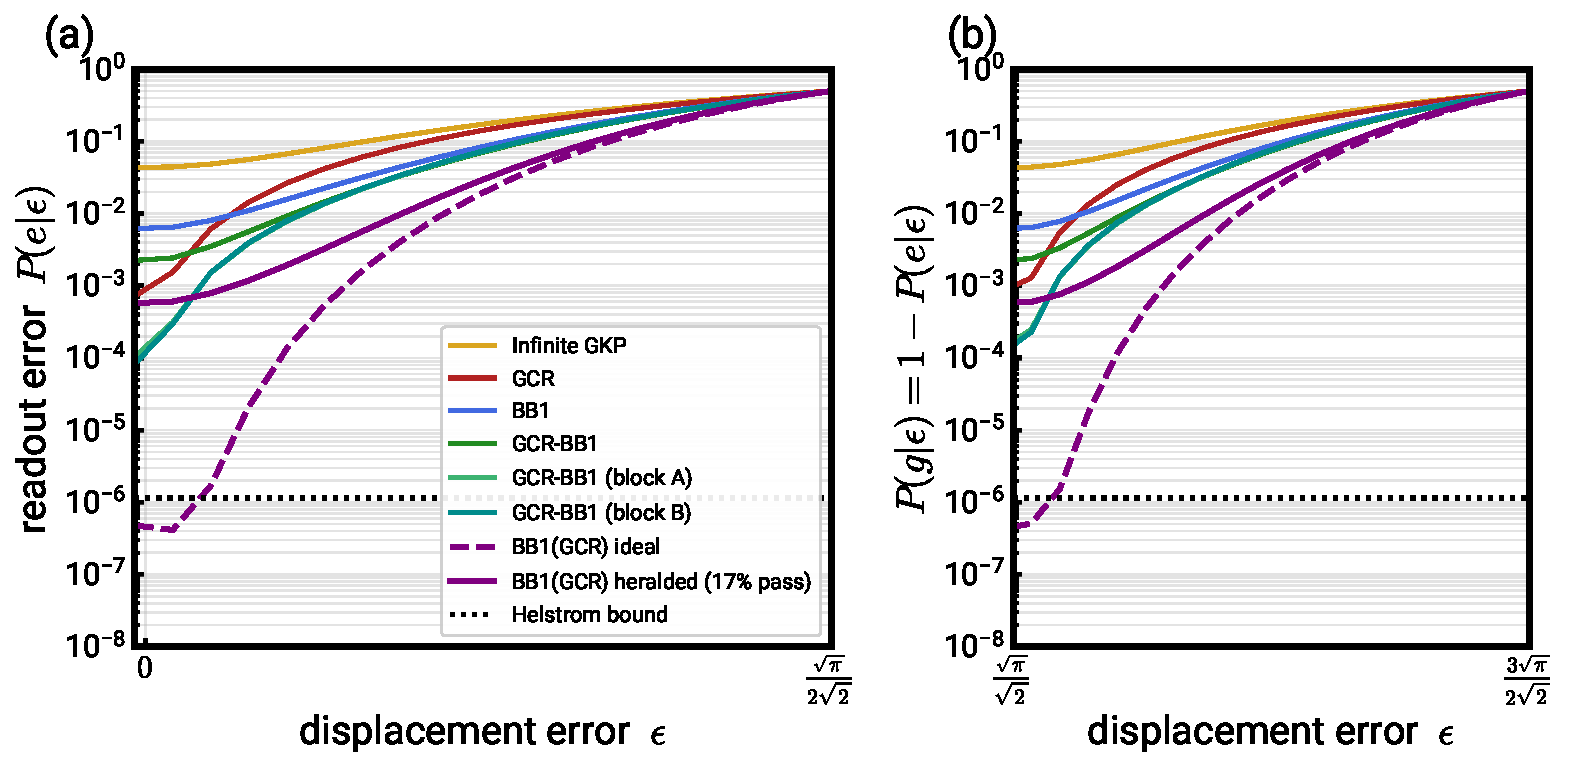
\includegraphics[width=\linewidth]{Paper_Figures/readout_combined.pdf}
\caption{\textbf{(a)} Readout error $P(e|\epsilon)$ vs displacement error $\epsilon$ for all GKP
readouts: infinite-energy (goldenrod), finite-energy GCR (firebrick), Abelian BB1 (royalblue),
GCR-BB1 (forestgreen), its two block variants (block~A, mediumseagreen; block~B, darkcyan), and
BB1(GCR) --- the non-unitary \emph{ideal} (purple dashed) and the
\emph{heralded} readout (purple solid, $\sim17\%$ herald pass). Dotted: the Helstrom bound
($\approx1.1\times10^{-6}$, computed from the two logical-codeword overlap at $\Delta=0.34$). The
ideal falls below Helstrom because it is a non-unitary
limit, not a deterministic measurement. \textbf{(b)} the \emph{logical-1} readout error
$P(g|\epsilon)=1-P(e|\epsilon)$ (log, same curves) over the logical-1 peak: it mirrors (a), dipping to
the floor at $\epsilon=\sqrt{\pi/2}$ (ideal $\sim10^{-10}$, heralded $\sim5.7\times10^{-4}$); the
Helstrom bound (dotted) again lies below only the ideal. The displacement error is in units of
$\sqrt{\pi}/2\sqrt2$ (ticks: panel (a) $\{0,\,\sqrt{\pi}/2\sqrt2\}$; panel (b)
$\{\sqrt{\pi}/\sqrt2,\,3\sqrt{\pi}/2\sqrt2\}$).}
\label{fig:readout}
\end{figure}

\subsection{On a failed herald: restart, reuse, and back-action}\label{sec:endofline}
This is an \emph{end-of-line} readout, so the oscillator is discarded afterwards. The back-action is
sharply \emph{conditional}: on a successful herald the completed readout is nearly QND --- the
oscillator returns to the input at fidelity $0.996$ (purity $0.999$), so the $\sim17\%$ good shots
preserve the state as well as reading the bit --- whereas the $\sim83\%$ failure branch destroys it
(oscillator fidelity $\approx0.24$, though the mean position $\langle\hat x\rangle$ is still
preserved). So the problem is not back-action per se, but that the destructive branch dominates. When
a herald fails, can one recover the sharp read? There are only two ways to try, and neither works.
The first would be to start again from the original oscillator state, but this is impossible: the
oscillator \emph{is} the unknown data being read, and there is no copy to re-prepare. (This is
precisely why the same heralding works cleanly in state preparation or calibration, where the input is
known and can simply be re-prepared, but not for a data readout.) The second would be to reuse the
disturbed oscillator with a fresh qubit. Here the coarse bit survives but the precision does not: a
failed correction herald applies the complementary non-unitary Kraus operator, which reweights the
wavefunction while leaving the mean position $\langle\hat x\rangle$ \emph{unchanged} at every peak, so
the correct \emph{sign} is still read. The \emph{sharpness}, however, is lost --- even a subsequently
successful restart gives only $P(-1)|_{x=0}\approx9\times10^{-2}$ after one failed round, already
\emph{worse} than the single bare BB1 ($6\times10^{-3}$) that BB1(GCR) was meant to improve, degrading
to $\sim0.15$ and $0.21$ after two and three. The non-unitary shear accumulates and re-correction does
not undo it; on the all-fail branch the oscillator's fidelity to the input is $\approx0.24$, and no
displacement or momentum boost recovers it.

The sharp $5.7\times10^{-4}$ read is thus a \emph{first-attempt} prize available only on the
$\sim17\%$ success branch, and because a failed attempt's back-action is destructive this is not a
scheme that can be ``repeated to increase fidelity'' --- that recourse applies only to readouts whose
back-action is small on \emph{every} outcome, such as single GCR or GCR-BB1. The practical verdict is
therefore negative: every use carries an $\sim\!83\%$ chance of leaving the oscillator in a state that
reads \emph{worse than bare BB1} and cannot be re-prepared, so the scheme destroys the logical
information more often than it sharpens it.
BB1(GCR) is a proof that the non-unitary correction is physically recoverable in post-selectable
settings, not a deployable readout.

\section{Calibration: realizing the ideal correction, and its noise budget}\label{sec:calibration}
The $\gtrsim83\%$ discard that rules BB1(GCR) out as a data readout is a property of reading
\emph{unknown} data, whose state cannot be re-prepared or copied. In \emph{calibration} --- where the
readout is characterized on a \emph{known}, re-preparable GKP state $\ket\psi$ --- those restrictions
lift, and the ideal (non-unitary) correction can be applied \emph{deterministically in expectation}.
We give the explicit protocol and, crucially, its noise budget: under realistic decoherence the two
natural routes differ by more than an order of magnitude, and the shot-optimal one is the wrong choice.

It helps to recognize what the correction is: each GCR correction
$M=e^{c\hat p\sigma_\phi}=e^{-\tau H_{\mathrm{eff}}}$ is a small imaginary-time step, with
$H_{\mathrm{eff}}=-\hat p\sigma_\phi$ a low-weight ``Hamiltonian'' and
$\tau=c=\eta\Delta^2/2|\alpha|\le0.41$, so any imaginary-time-evolution method applies. The
noise-sensible route is simply repeat-until-success. Because $\ket\psi$ is re-preparable, the
deterministic-in-expectation realization needs \emph{no} amplitude amplification: we prepare $\ket\psi$,
run the \emph{shallow} heralded BB1(GCR) of Sec.~\ref{sec:flagged} (one composite pulse, eight
conditional displacements, $\sim\!6\,\mu\mathrm{s}$), and keep the shot if the heralds fire; otherwise
re-prepare and retry. Heralding three corrections passes with $P_{\mathrm{succ}}\approx17\%$
($\sim\!6$ attempts; floor $5.7\times10^{-4}$), and heralding all four returns the ideal response
($4\times10^{-7}$) at $\approx7\%$ ($\sim\!14$ attempts). This pass rate is essentially
\emph{noise-independent}: tracking the un-normalized norm against the subspace bound
($\lambda\approx7.2$ on $n\le40$) gives $17.3\%\to17.6\%$ under the system channels --- decoherence
reshapes the state toward larger $\|M\ket\psi\|^2$ --- while the opposite-sign ancilla-flip effect is
small ($\sim\!1$--$2\%$), so the average retry count stays $\sim\!6$ (three heralds) and $\sim\!14$
(all four) in the presence of noise. The cost is \emph{wall-clock attempts, not
coherence depth}: each coherent circuit is a single $\sim\!6\,\mu\mathrm{s}$ pulse, and failed attempts
--- with all their decoherence --- are discarded. Decoherence thus costs accepted-shot fidelity
($\sim\!3\%$ below), not yield. Fast, high-fidelity re-preparation of the GKP
codeword (the GCR-based scheme of the main text) makes the retries cheap, and the idle state can be
kept alive between attempts by stabilizing with a \emph{separate} ancilla in the quadrature orthogonal
to the read-out displacement $\epsilon$, leaving the measured quantity untouched.

To quantify the noise budget of one accepted shot, we simulate a single accepted RUS shot on the full GKP
codeword ($\langle n\rangle=6$) with a gate-level Kraus model under the experimental error rates of
Sivak \emph{et al.}\ (Nature \textbf{616}, 50 (2023)): transmon and ancilla
$T_1=T_\phi=200\,\mu\mathrm{s}$, cavity $T_1=1000\,\mu\mathrm{s}$. Decoherence is applied after each
conditional displacement, whose duration equals its amplitude (an amplitude-$1$ CD takes
$1\,\mu\mathrm{s}$; the eight gates total $\sim\!6\,\mu\mathrm{s}$, with the two large position kicks
dominating and the small-amplitude corrections nearly instantaneous), and the herald is post-selected.
The exact ideal correction sets a noiseless floor of $6\times10^{-4}$; decoherence adds
\begin{center}
\begin{tabular}{lc}
\toprule
error channel & readout-infidelity increment\\
\midrule
transmon decay & $+2.0\%$\\
transmon dephasing & $+0.7\%$\\
cavity photon loss & $+0.5\%$\\
ancilla decay / dephasing & $<0.05\%$ (herald-protected)\\
\midrule
\textbf{all channels} & $\boldsymbol{\approx3\%}$\\
\bottomrule
\end{tabular}
\end{center}
The accepted-shot readout infidelity is $\approx3\%$, dominated by transmon \emph{decay} over the
$\sim\!6\,\mu\mathrm{s}$ circuit (the $2\pi$ position kick, $|\beta|\!\approx\!2.5$, is by far the
longest gate); dephasing and cavity loss are sub-percent because the corrections are fast
small-amplitude gates, and \emph{ancilla errors are caught by the
herald} --- they flip the flag and lower the yield rather than corrupting accepted shots, a built-in
error-detection benefit of the flagged construction (and the reason the ancilla channels barely
register above). Averaging over the many shots a calibration already takes reduces this further.

Amplitude amplification, by contrast, is shot-efficient but coherence-infeasible. One can instead render a
\emph{single} coherent circuit deterministic by amplitude amplification. Let $V$ be the block-encoding
of the full correction (the per-pulse gadgets of Sec.~\ref{sec:herald-gates} interleaved with the
position kicks), acting on $\ket\psi$ and a herald ancilla $\ket0_a$:
\begin{equation}
V\,\ket0_a\ket\psi \;=\; a\,\ket0_a\frac{M\ket\psi}{\|M\ket\psi\|}\;+\;\sqrt{1-a^2}\,\ket{\Phi^\perp},
\qquad a=\frac{\|M\ket\psi\|}{\lambda}=\sqrt{P_{\mathrm{succ}}}.
\end{equation}
Because $\ket\psi$ is known, both reflections are available,
\begin{align}
R_a &= I - 2\,\ket0_a\!\bra0_a &&\text{(reflect about herald success),}\\
R_\psi &= V\,\big(I - 2\,\ket0_a\ket\psi\bra\psi\bra0_a\big)\,V^\dagger
      &&\text{(reflect about the input),}
\end{align}
and $k\approx \pi/(4\arcsin a)-\tfrac12$ rounds of the Grover operator $G=-R_\psi R_a$ rotate the
amplitude to unity: from $a=0.27$ (four corrections) and $a=0.42$ (three) this is $k\approx3$ and
$k\approx2$ rounds. This is \emph{shot-optimal} --- three rounds rather than fourteen retries. But each
round requires the input reflection $R_\psi$, which \emph{un-prepares and re-prepares} $\ket\psi$
\emph{coherently}; three rounds therefore stack $\sim\!3\times$ a full GKP preparation into one coherent
circuit of $\sim\!130\,\mu\mathrm{s}$ --- comparable to $T_1$. A gate-count Kraus budget then gives
per-channel exponents $\gamma T\approx\kappa\langle n\rangle T\approx0.7$--$0.9$ and a \emph{total
readout infidelity $\approx0.98$}: the readout is destroyed by decoherence. The determinism is bought
with depth --- exactly the wrong trade when the error accrues per unit time:
\begin{center}
\begin{tabular}{lccc}
\toprule
route & coherent depth & attempts & total infidelity\\
\midrule
repeat-until-success & $\sim\!6\,\mu\mathrm{s}$ & $\sim\!6$--$14$ & $\approx3\%$\\
amplitude amplification & $\sim\!130\,\mu\mathrm{s}$ & $1$ & $\approx0.98$\\
\bottomrule
\end{tabular}
\end{center}
Fixed-point amplitude amplification (Yoder, Low, and Chuang, PRL \textbf{113}, 210501 (2014)) removes
the need to know $a$ in advance but not the reflections, so it does not change this verdict.

Three single-unitary routes avoid the input reflection $R_\psi$ altogether, each compiling $M$ into
one deterministic unitary. The first is a linear combination of unitaries: $e^{c\hat p}$ is a
Gaussian-weighted combination of real displacements (Hubbard--Stratonovich), so $M$ is an LCU with
$1$-norm $\lambda\approx3.8$, and its $\mathrm{PREPARE}$--$\mathrm{SELECT}$ circuit, amplified as above,
gives $O(\lambda)$ deterministic queries. The second is multi-copy imaginary-time evolution
(Schwartzman \emph{et al.}, arXiv:2603.11208), in which a few copies of $\ket\psi$, real-time
evolution under $H_{\mathrm{eff}}$, and controlled-SWAPs realize $e^{-\tau H_{\mathrm{eff}}}$ by a
\emph{unitary} circuit with no post-selection and no input reflection; the copy count is set by the
order needed to reach $\tau\|H_{\mathrm{eff}}\|_{\mathrm{eff}}\sim c/\Delta\sim1.2$, i.e.\ a handful.
The third is variational QITE (McArdle \emph{et al.}, npj Quantum Inf.\ \textbf{5}, 75 (2019)): since
$H_{\mathrm{eff}}=\hat p\sigma_\phi$ is low-weight, the ansatz is small and compiles to a fixed
deterministic unitary at moderate measurement cost, and Sec.~\ref{sec:qite-readout} quantifies what
such a compilation achieves when used directly as a \emph{stand-alone deterministic readout}. If any of
these unitaries has a depth closer to the RUS pulse than to the amplification circuit, it could combine
determinism with a tolerable noise budget --- the only regime in which a strictly deterministic
calibration would be worthwhile.

In scope, every route here needs the input known, re-preparable, or copyable --- available in
calibration but forbidden for single-shot readout of unknown data by no-cloning. Under realistic
decoherence the practical calibration tool is repeat-until-success ($\approx3\%$ per accepted shot,
reduced further by averaging); amplitude amplification, though shot-optimal, is ruled out by its
$\sim\!130\,\mu\mathrm{s}$ coherent depth.

\section{A deterministic readout by variational compilation, and the noise-limited verdict}
\label{sec:qite-readout}
The calibration routes of Sec.~\ref{sec:calibration} realize the \emph{exact} $M$. But a
fault-tolerant readout does not need the ideal floor --- it needs only to sit below the code's
threshold ($\sim\!10^{-2}$). This sharpens the question: what is the best \emph{deterministic}
readout (a single unitary, no post-selection, no discard, no re-preparation) that a \emph{short}
conditional-displacement circuit can achieve? If a shallow unitary already clears threshold, the
entire heralding apparatus is unnecessary \emph{for the readout}.

To answer this, we keep the BB1(GCR) position kicks fixed and replace each
non-unitary correction by a \emph{deterministic} momentum correction $C_k=e^{-i c_k\hat p\sigma_{\nu_k}}$,
then optimize the amplitudes and axes $\{c_k,\nu_k\}$ --- a QITE-style compilation of the imaginary-time
step into a fixed unitary --- to minimize the readout error, correctly reading logical-$0$ (at
$\epsilon=0$) as $+1$ and logical-$1$ (at $\epsilon=2u=\sqrt{\pi/2}$) as $-1$. We seed from the
analytic GCR values --- amplitude $c_k=\theta_k\Delta^2/2|\alpha|$ and realizability axis
$\sigma_\gamma=\hat n\times\hat\phi$ (i.e.\ $\nu_k=\phi_k+\pi/2$) --- and then \emph{grow} additional
deterministic correction layers to test whether depth helps.

Contrasting the analytic GCR values (what the correction \emph{should} be) with the compiled optimum
(what actually minimizes the readout error) exposes two systematic moves (Table~\ref{tab:qite}). The
first concerns the axes: the three corrections rotate by $\approx\pi/2$ \emph{off}
the GCR-prescribed $\hat n\times\hat\phi$ axis, landing on the position-kick axis $\sigma_{\phi_k}$
itself --- which is exactly the axis of the \emph{ideal} non-unitary $M=e^{c\hat p\sigma_\phi}$. The
best unitary correction thus points along the ideal $M$'s own axis, \emph{not} along the
realizability-rule axis that makes the physical unitary GCR wash out (Tables~\ref{tab:cases}); re-pointing
onto $\sigma_\phi$ is precisely how the compiled readout escapes that washout. The target $C_4$ instead
stays near its seed $\sigma_y$. The second concerns the amplitudes: the strong $2\pi$ correction is \emph{damped} from
$4$ to $2.9$ (a full-strength unitary over-rotates at that angle --- point (ii) above), while the target
is \emph{boosted} from $1$ to $2.5$; the two nominally identical $\pi$ corrections even emerge asymmetric
($2.5$ vs $1.6$). The optimizer keeps the GCR geometry only loosely --- it re-points onto the ideal axis
and re-weights --- but a norm-preserving gate can neither reproduce $M$'s contraction nor beat the
$1.5\times10^{-3}$ plateau.
\begin{table}[h]
\centering
\begin{tabular}{lcccc}
\toprule
 & \multicolumn{2}{c}{amplitude $c_k$ $[\,|\alpha|\Delta^2\,]$} & \multicolumn{2}{c}{axis $\nu_k$ $[\,\pi\,]$}\\
correction & GCR & compiled & GCR & compiled\\
\midrule
$C_1$ ($\pi$)          & $2$ & $2.5$ & $0.04$ & $0.60$\\
$C_2$ ($2\pi$)         & $4$ & $2.9$ & $0.12$ & $0.61$\\
$C_3$ ($\pi$)          & $2$ & $1.6$ & $0.04$ & $0.55$\\
$C_4$ (target $\pi/2$) & $1$ & $2.5$ & $0.50$ & $0.40$\\
\bottomrule
\end{tabular}
\caption{Deterministic corrections $C_k=e^{-ic_k\hat p\sigma_{\nu_k}}$: the analytic GCR prescription
versus the QITE-compiled optimum. Amplitudes $c_k$ in units of $|\alpha|\Delta^2$ (the GCR value is
$\theta_k\Delta^2/2|\alpha|=(2\theta_k/\pi)\,|\alpha|\Delta^2$, i.e.\ $\{2,4,2,1\}$); axes $\nu_k$ in
units of $\pi$ as headless equatorial directions $\sigma_\nu$ (mod $\pi$), with the GCR value
$\nu_k=\phi_k+\pi/2=\hat n\times\hat\phi$. The corrections rotate $\approx\pi/2$ onto the kick axis
$\sigma_{\phi_k}$ (the ideal-$M$ axis) and the $2\pi$ amplitude is damped $4\!\to\!2.9$.}
\label{tab:qite}
\end{table}

The result is a plateau, well above the ideal.
\begin{center}
\begin{tabular}{lc}
\toprule
deterministic readout & readout error\\
\midrule
bare single conditional displacement & $4.5\times10^{-2}$\\
bare BB1 (composite, no GCR correction) & $7.5\times10^{-3}$\\
physical det.\ BB1(GCR) ($\sigma_y$ on all four) & $0.49$ (washes out)\\
single GCR (target pulse only) & $2.6\times10^{-3}$\\
\textbf{optimized deterministic ansatz} & $\boldsymbol{1.5\times10^{-3}}$\\
\quad $+1$ correction layer & $1.5\times10^{-3}$\\
\quad $+2$ correction layers & $1.5\times10^{-3}$\\
\midrule
heralded / ideal (post-selected) & $5.7\times10^{-4}$\\
Helstrom bound & $1.1\times10^{-6}$\\
\bottomrule
\end{tabular}
\end{center}
The optimized deterministic readout reaches $1.5\times10^{-3}$ --- a factor $\sim\!5$ better than bare
BB1 ($7.5\times10^{-3}$, the composite pulse the correction is added to) and $\sim\!1.7$ better than a
single GCR --- and it \emph{escapes} the physical washout ($0.49$) that a fixed $\sigma_y$ correction on
all four pulses suffers. But it \emph{plateaus}: adding correction layers does not lower it. (This
accuracy sweep uses $N_{\mathrm{cav}}=40$ for optimizer tractability; at the $N_{\mathrm{cav}}=100$ of
the noise simulations single GCR and the optimized ansatz both converge to $\approx1.4\times10^{-3}$,
and the plateau persists.) The
shallow conditional-displacement class therefore saturates a factor $\sim\!3$ above the herald's ideal
floor and four orders of magnitude above the Helstrom bound. The gap below the finite-energy floor is
exactly what the \emph{non-unitary} contraction of Sec.~\ref{sec:flagged} buys and a norm-preserving
unitary cannot; a Helstrom-saturating deterministic measurement exists in principle but requires a
deep, non-local circuit outside this local ansatz. This is the note's central conclusion reached from
the deterministic side: no short unitary matches the heralded floor.

These coherent floors are, however, largely academic under realistic decoherence, where accounting for
gate \emph{durations} overturns the ranking altogether --- length, not accuracy, decides. A
conditional displacement of amplitude $|\beta|$ takes $|\beta|\,\mu\mathrm{s}$ (an amplitude-$1$ CD is
$1\,\mu\mathrm{s}$), so a readout's cost is set by its \emph{position kicks}; the corrections are
tiny-amplitude ($|\beta|\lesssim0.3$) and nearly free. The full BB1(GCR) is dominated by its $2\pi$ kick
($|\beta|\!\approx\!2.5$, i.e.\ $2.5\,\mu\mathrm{s}$) --- a gate it \emph{shares with bare BB1} ---
whereas single GCR omits it, using only the $\theta_\mathrm{t}=\pi/2$ kick. At the rates of
Sec.~\ref{sec:calibration}:
\begin{center}
\begin{tabular}{lcccc}
\toprule
readout & circuit time & coherent floor & noise & total\\
\midrule
\textbf{single GCR} & $0.7\,\mu\mathrm{s}$ & $1.4\times10^{-3}$ & $+0.2\%$ & $\boldsymbol{\approx0.4\%}$\\
bare BB1 & $5.6\,\mu\mathrm{s}$ & $6.4\times10^{-3}$ & $+2.6\%$ & $\approx3.2\%$\\
BB1(GCR), deterministic & $6.3\,\mu\mathrm{s}$ & $1.5\times10^{-3}$ & $+3.2\%$ & $\approx3.2\%$\\
BB1(GCR), heralded & $6.3\,\mu\mathrm{s}$ & $5.7\times10^{-4}$ & $+3.2\%$ & $\approx3.2\%$ ($17\%$ yield)\\
\bottomrule
\end{tabular}
\end{center}
Two things follow. First, BB1(GCR) is essentially \emph{bare BB1} under noise: the GCR correction
lowers the coherent floor by an order of magnitude ($6.4\times10^{-3}\!\to\!6\times10^{-4}$) at almost
no extra circuit time ($+0.7\,\mu\mathrm{s}$, $+12\%$) --- the corrections are essentially free --- but
the $\sim\!3\%$ noise, set by the \emph{shared} kicks, masks the gain entirely, so both land at
$\approx3.2\%$. Second, single GCR wins by $\sim\!8\times$: dropping the long $2\pi$ kick makes it a
$0.7\,\mu\mathrm{s}$ circuit, so decoherence adds only $\sim\!0.2\%$, and its coherent floor
($1.4\times10^{-3}$) already \emph{equals} the deterministic plateau, so it sacrifices no accuracy to
get there. Under realistic noise the shortest adequate readout dominates.

The practical choice for a \emph{noisy} GKP readout is therefore \textbf{single GCR} ---
$\approx\!0.4\%$, deterministic, discard-free, and the shortest circuit that clears threshold. The elaborate BB1(GCR) machinery (the $2\pi$ correction, heralding,
post-selection) delivers its lower coherent floor only in a low-noise limit today's hardware does not
reach: its advantage over bare BB1 and single GCR stays masked until the per-shot decoherence drops
below the coherent gap, $\sim\!10^{-3}$ (an order of magnitude better coherence than assumed here).
BB1(GCR)'s roles are thus (a) the high-coherence / noiseless-limit readout; (b) the certification tool
that fixes the deterministic readout's floor; and (c) the high-fidelity primitive for known-state
preparation and calibration (Sec.~\ref{sec:calibration}), where re-preparation is free and the
$5.7\times10^{-4}$--$4\times10^{-7}$ accuracy is the whole point. For end-of-line data readout on
current devices, single GCR is the better choice.

\section{Readout under realistic noise: master-equation simulation}\label{sec:mesolve}
The gate-count budget of Sec.~\ref{sec:qite-readout} is confirmed and extended by a full
master-equation (\texttt{mesolve}) simulation at $N_{\mathrm{cav}}=400$. Each conditional displacement
of amplitude $|\beta|$ is evolved for a duration $|\beta|\,\mu\mathrm{s}$ (amplitude-$1$ CD $=1\,\mu$s)
under the experimental collapse operators (transmon and ancilla decay and dephasing
$T_1=T_\phi=200\,\mu\mathrm{s}$; oscillator photon loss $T_1=1000\,\mu\mathrm{s}$). We simulate seven
readouts --- single GCR, the QITE-compiled deterministic BB1(GCR), bare BB1, GCR-BB1 (bare BB1 preceded
by a single QITE-optimized momentum pre-correction), two \emph{block} variants that prepend four momentum
pre-corrections (block~A, block~B), and the heralded BB1(GCR)
--- isolating each channel and the total across the two Fig-3 displacement-error windows
(Fig.~\ref{fig:seq}; readout error in Fig.~\ref{fig:paired-readout}, oscillator infidelity in
Fig.~\ref{fig:paired-infidelity}).

Consider the readout error first. At the operating point, under all channels,
\begin{center}
\begin{tabular}{lcc}
\toprule
readout & full-noise error & dominant channel\\
\midrule
\textbf{single GCR} & $\boldsymbol{3.3\times10^{-3}}$ & transmon decay\\
BB1(GCR), deterministic & $2.2\times10^{-2}$ & transmon decay\\
GCR-BB1 (one pre-correction) & $2.4\times10^{-2}$ & transmon decay\\
GCR-BB1 (block A) & $2.4\times10^{-2}$ & transmon decay\\
GCR-BB1 (block B) & $2.4\times10^{-2}$ & transmon decay\\
bare BB1 & $2.8\times10^{-2}$ & transmon decay\\
heralded BB1(GCR) & $3.7\times10^{-2}$ & transmon decay\\
\bottomrule
\end{tabular}
\end{center}
confirming the verdict of Sec.~\ref{sec:qite-readout}: single GCR is $\sim\!8\times$ more accurate than
the full-length schemes because it is the shortest circuit (it omits the long $2\pi$ kick), and the bit
error is set by transmon decoherence over the circuit --- oscillator loss barely touches the readout
qubit ($+6\times10^{-4}$ for GCR).

The oscillator back-action turns out to be a \emph{recoverable} displacement rather than genuine
damage. The post-read oscillator stays nearly \emph{pure} (impurity $1-\mathrm{Tr}\rho^2\approx1$--$18\%$,
growing with circuit length), yet its \emph{raw} overlap with the input codeword is only $\sim\!0.5\%$ (fidelity
$F\approx0.07$). These are reconciled by a single fact: the read applies a large, \emph{state-agnostic}
displacement --- the conditional-displacement pulses kick the oscillator by an amount fixed by the
qubit, \emph{independent of the oscillator's location}. Calibrating this displacement \emph{once} on the
no-error logical-$0$ readout output,
\begin{equation}
\beta_{\mathrm{corr}}=+\,i\,\tfrac{1}{2}\sqrt{\pi/2}\qquad(\text{a pure momentum shift}),
\end{equation}
and applying $D(\beta_{\mathrm{corr}})$ to \emph{every} input --- the corrective displacement used in the
readout itself --- recovers the oscillator fidelity from $F\approx0.07$ to
\begin{center}
\begin{tabular}{lcc}
\toprule
readout & noiseless $F$ & full-noise $F$\\
\midrule
\textbf{single GCR} & $0.974$ & $\mathbf{0.971}$\\
GCR-BB1 (one pre-correction) & $0.977$ & $0.953$\\
GCR-BB1 (block A) & $0.977$ & $0.951$\\
GCR-BB1 (block B) & $0.976$ & $0.950$\\
bare BB1 & $0.975$ & $0.951$\\
BB1(GCR), deterministic & $0.960$ & $0.933$\\
heralded BB1(GCR) & $0.974$ & $0.926$\\
\bottomrule
\end{tabular}
\end{center}
flat across the $\epsilon$ window. So the oscillator is $\sim\!93$--$97\%$ preserved per read after one
calibrated corrective displacement --- the apparent near-orthogonality was entirely this recoverable
kick, not decoherence --- and, as with the readout error, \emph{single GCR preserves it best under
noise} ($0.971$), its short circuit accruing the least decoherence while the longer BB1(GCR) drops to
$0.933$. The residual $\sim\!5\%$ (GCR) is a genuinely non-Gaussian distortion: neither a further
displacement nor a squeeze removes it (the optimal corrective squeeze is exactly zero), consistent with
the irreducible measurement back-action of extracting the bit. Appending small-Big-small stabilization
rounds to the post-read state does \emph{not} reduce this residual --- it is not a lattice displacement,
the only error such stabilization corrects --- so the corrective displacement is the operative and
sufficient mechanism. The only further gain available is combining \emph{repeated} GCR reads (two reads
log-odds-combined reach $\sim\!2\times10^{-6}$).

A fourth deterministic option sharpens the interpretation of what the GCR correction actually buys.
GCR-BB1 keeps the four bare BB1 kicks but prepends a \emph{single} conditional momentum displacement
$e^{-i c\hat p\sigma_\nu}$, whose two parameters we optimize by the same QITE search used for the
interleaved corrections (Sec.~\ref{sec:qite-readout}). The optimizer improves this lone pre-correction
sharply --- readout error $1.6\times10^{-2}\!\to\!2.3\times10^{-3}$, a $\sim\!7\times$ gain --- by
slightly enlarging its amplitude and tilting its axis $\sim\!9^\circ$ off $\sigma_\mathrm{y}$, the same
rotation-toward-the-kick-axis we saw in Table~\ref{tab:qite}. Because that pre-correction is a
$\sim\!0.02\,\mu\mathrm{s}$ gate against the $\sim\!5.6\,\mu\mathrm{s}$ of kicks it \emph{shares with bare
BB1}, GCR-BB1 carries essentially bare BB1's length, and hence its decoherence floor --- yet it sits
strictly above bare BB1 everywhere: lower readout error (noiseless $2.1\times10^{-3}$ vs
$6.1\times10^{-3}$; full-noise $2.4\times10^{-2}$ vs $2.8\times10^{-2}$) and higher fidelity in both
windows. Most tellingly, in the discriminating logical-$1$ window it \emph{beats the fully interleaved
deterministic BB1(GCR)} ($F=0.915$ vs $0.903$ under noise), because it pays for one correction rather
than four: a single well-placed QITE-tuned pre-kick captures most of the coherent benefit at a fraction
of the added machinery. Under noise it remains, like every full-length scheme, behind single GCR --- but
it is the clearest statement that the corrections want to be \emph{few and well-placed}, not numerous.

This invites the converse question: whether a \emph{block} of well-placed pre-corrections, rather than a
single one, can recover the interleaved scheme's coherent floor without paying its interleaved length. We
test two such blocks that prepend \emph{four} momentum corrections ahead of the bare BB1 kicks --- block~A,
a free QITE-optimized momentum-BB1 block, and block~B, the interleaved BB1(GCR) corrections analytically
conjugated to the front and then QITE-polished. Both slash the noiseless readout error to
$6.7\times10^{-5}$ (A) and $4.5\times10^{-5}$ (B), recovering $\sim\!30$--$47\times$ of the
single-pre-correction gap yet remaining $\sim\!5$--$7\times$ above the fully interleaved BB1(GCR)
($9.8\times10^{-6}$). Under realistic noise, however, the blocks carry the same full BB1 kick length and
hence the same $\sim\!2.4\times10^{-2}$ decoherence floor as GCR-BB1 and bare BB1 --- the coherent gain
washes out entirely. The block therefore trades a slightly longer prefix for a markedly lower
\emph{noiseless} floor without matching interleaving, and confirms once more that under decoherence the
corrections that matter are few and well-placed, not numerous.

\begin{figure}[tbp]
\centering
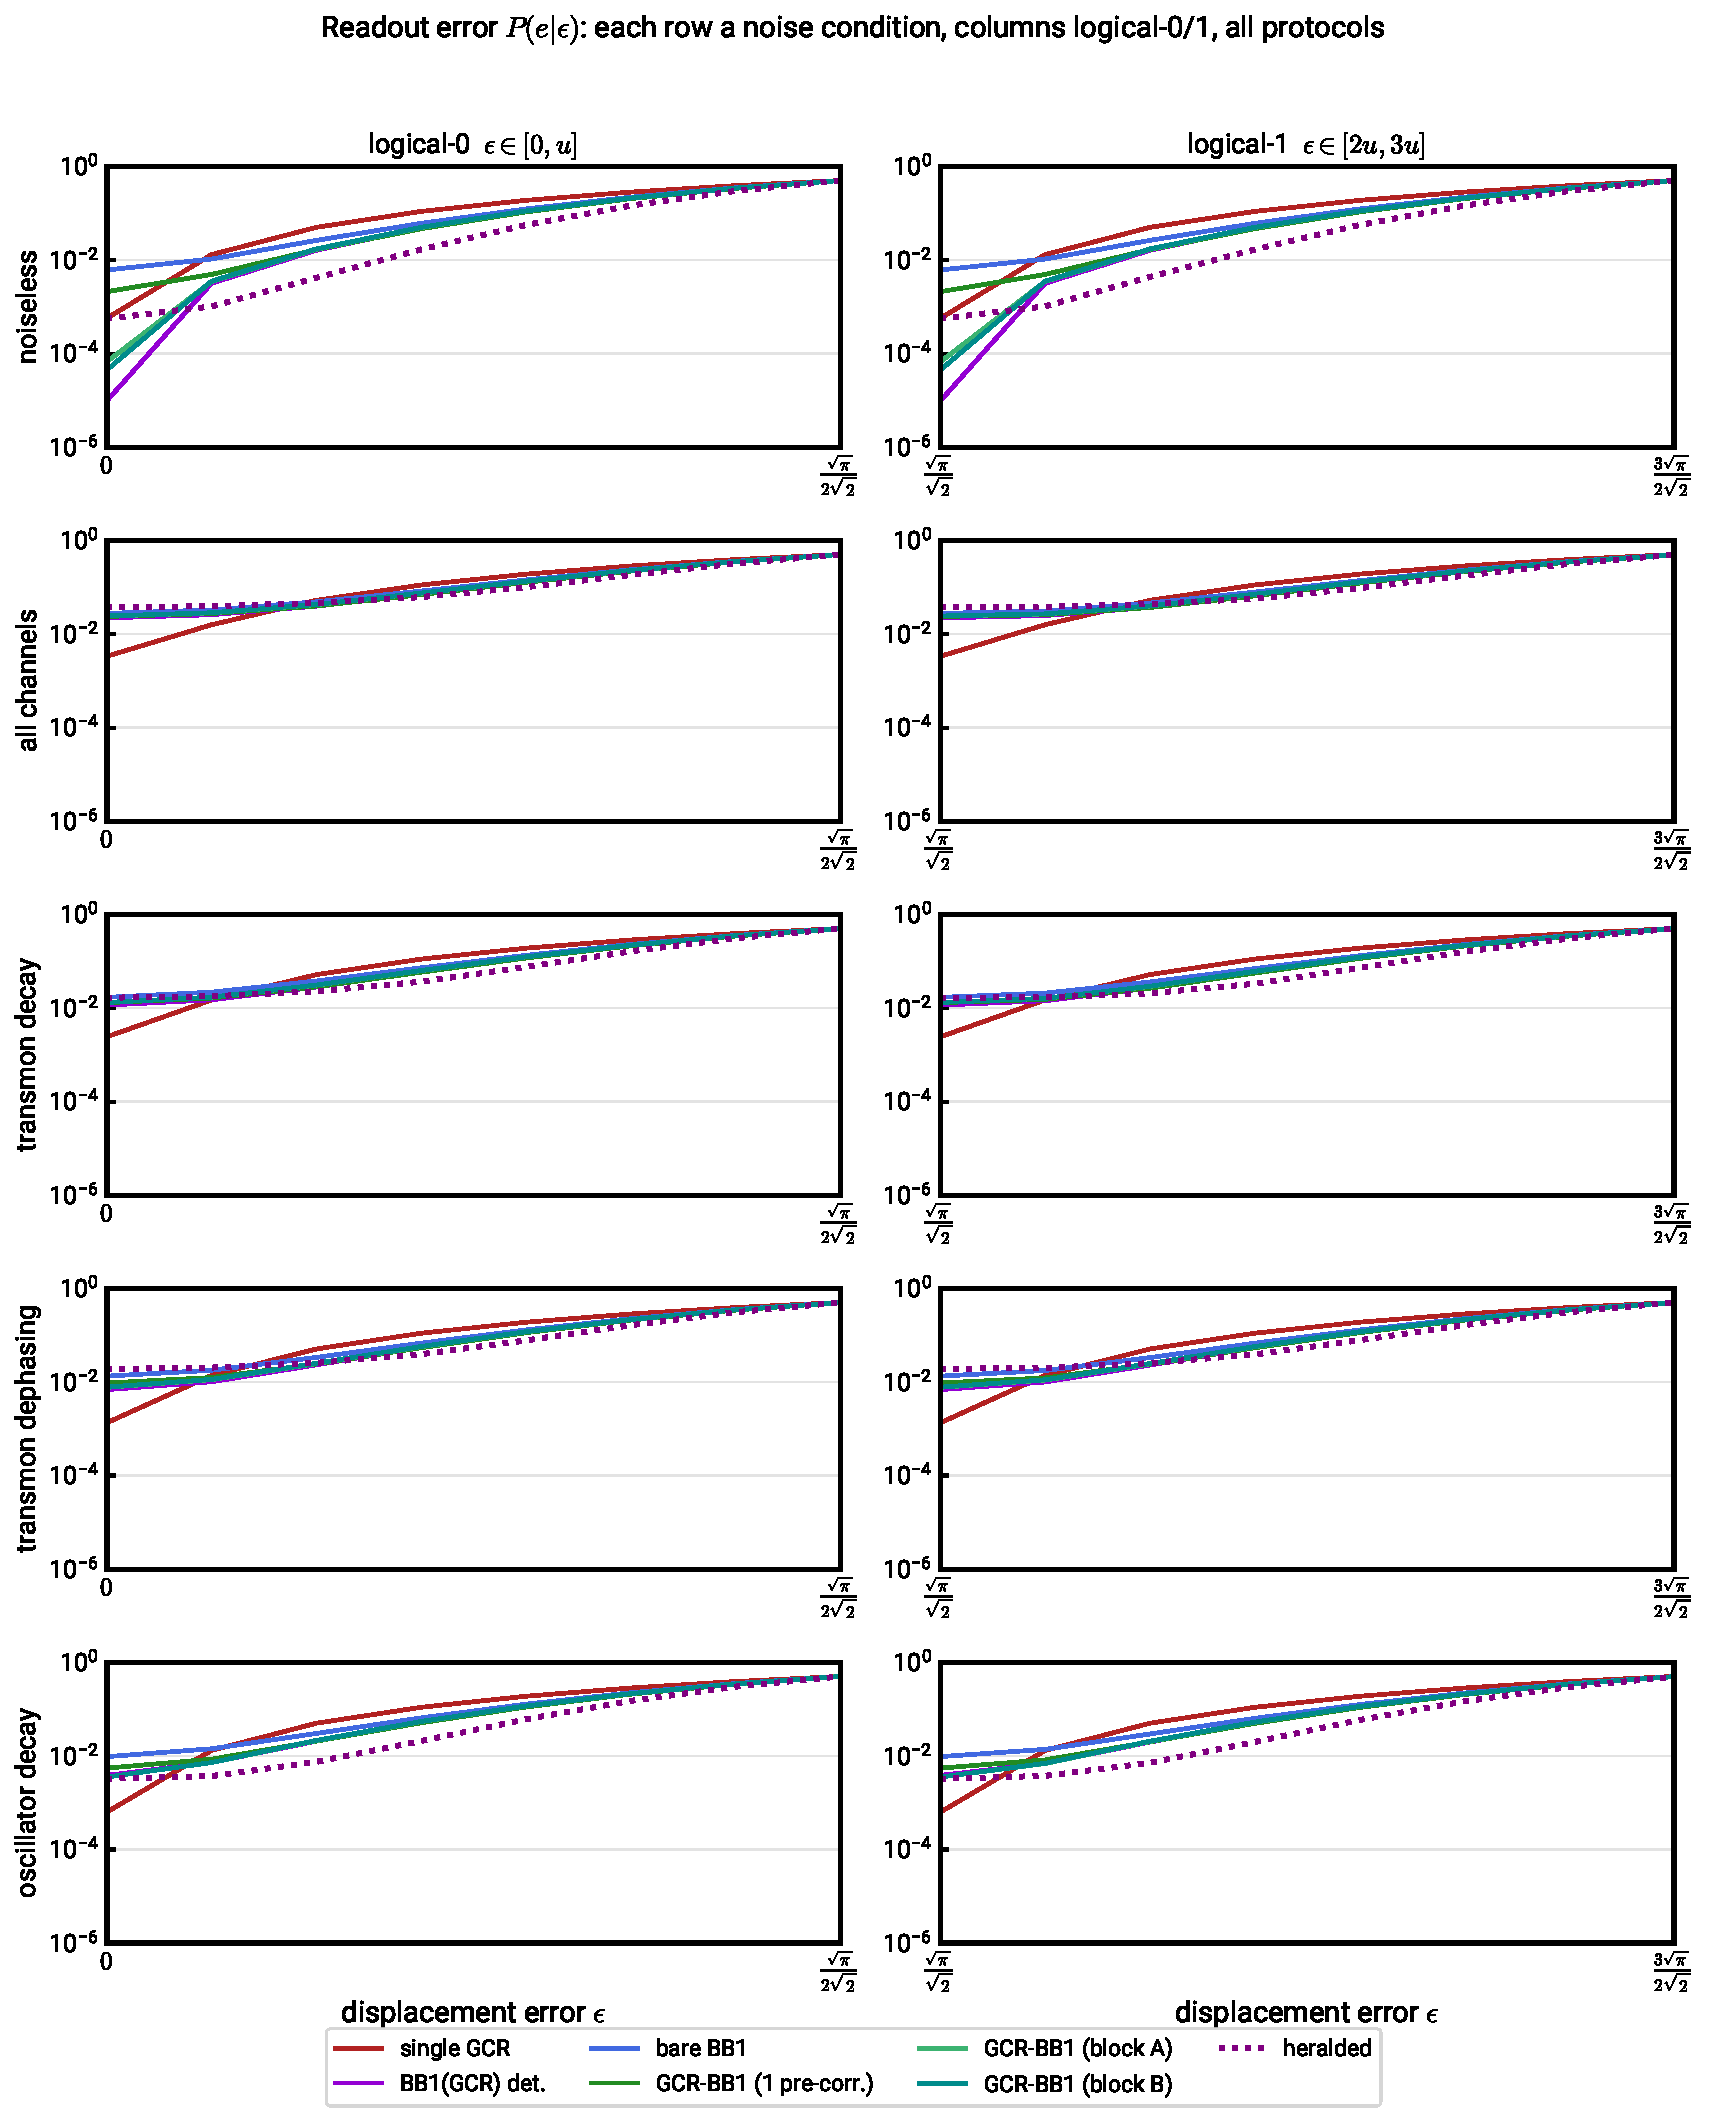
\includegraphics[width=0.82\textwidth]{Paper_Figures/mesolve_paired_readout.pdf}
\caption{Master-equation readout error $P(e|\epsilon)$ vs.\ displacement error $\epsilon$ for the seven
readouts: single GCR (red), deterministic BB1(GCR) (violet), bare BB1 (blue), GCR-BB1 (teal),
GCR-BB1 block~A (mediumseagreen) and block~B (darkcyan), heralded (purple, dotted). Rows are noise settings (noiseless; all channels; transmon decay; transmon
dephasing; oscillator decay); columns are the logical-$0$ ($\epsilon\in[0,u]$) and logical-$1$
($\epsilon\in[2u,3u]$) windows, $u=\sqrt{\pi}/(2\sqrt2)$. Noiseless, BB1(GCR) reaches $\sim\!10^{-5}$
(near-Helstrom); under decoherence all full-length schemes converge to a $\sim\!2$--$3\times10^{-2}$
floor set by circuit time, while the short single-GCR read stays $\sim\!8\times$ lower. GCR-BB1 (teal)
and its block variants (green/cyan) track bare BB1 but lie consistently below it; the blocks reach the
lowest noiseless floor of the deterministic schemes.}
\label{fig:paired-readout}
\end{figure}

\begin{figure}[tbp]
\centering
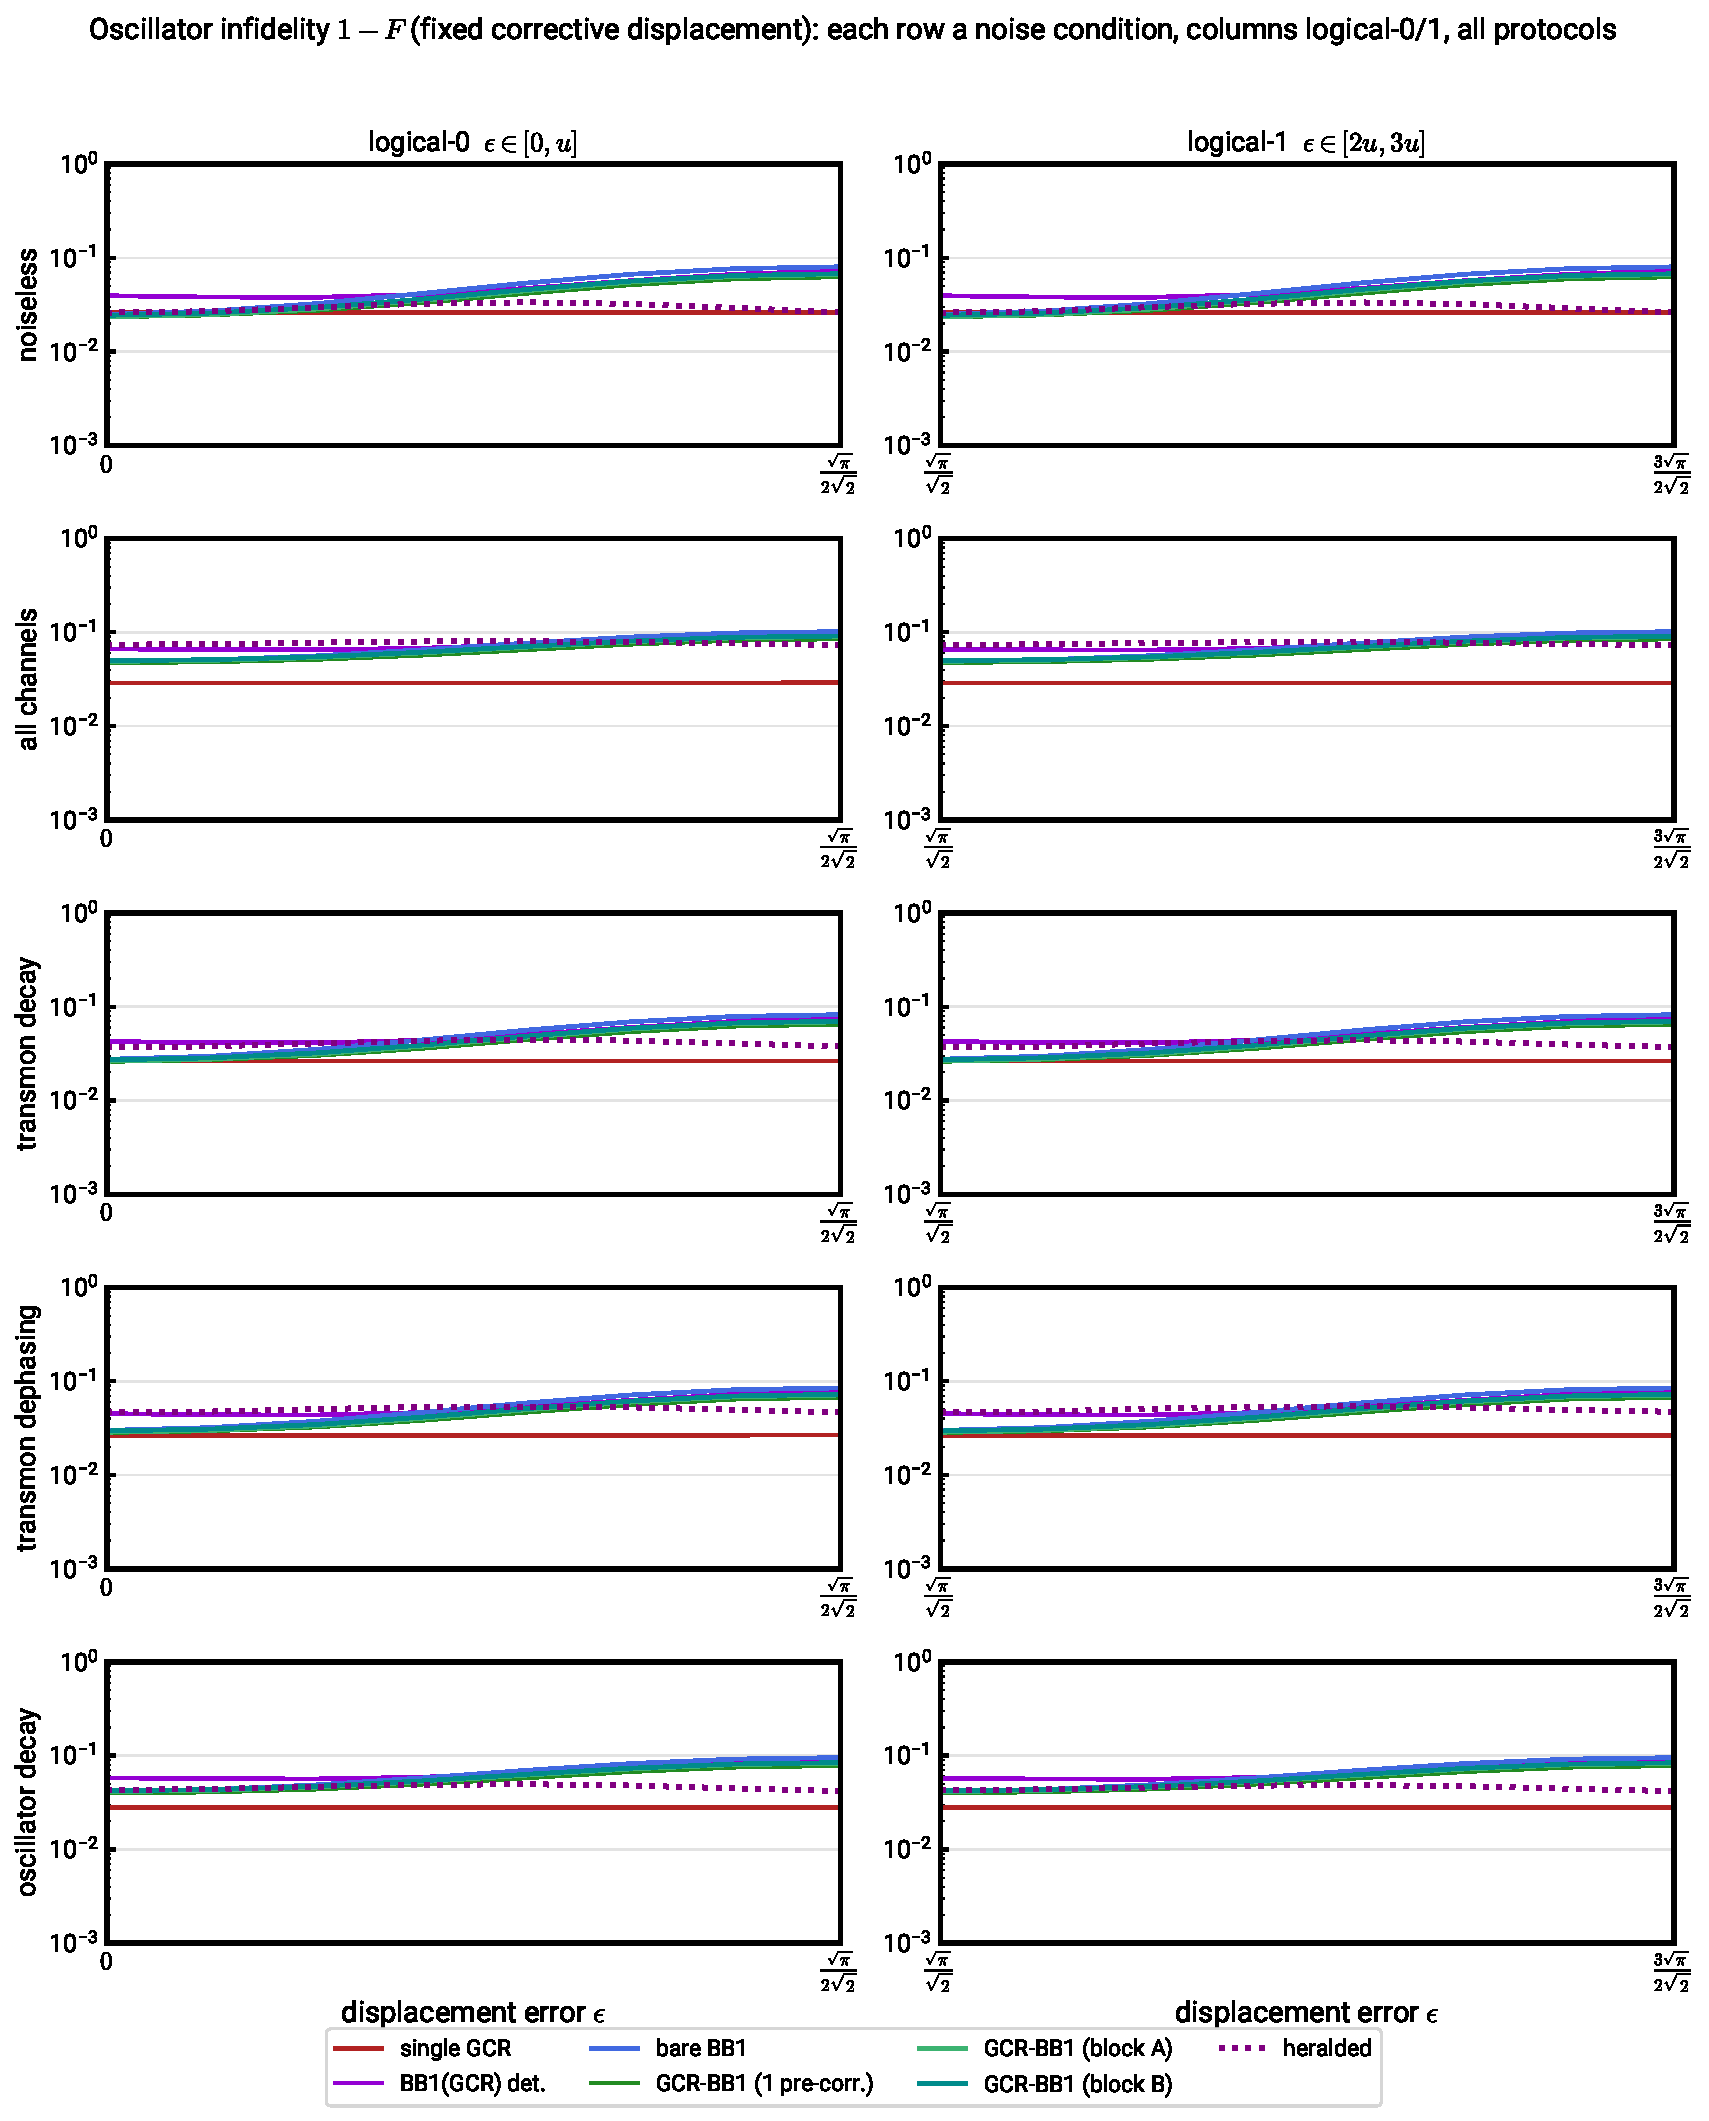
\includegraphics[width=0.82\textwidth]{Paper_Figures/mesolve_paired_infidelity.pdf}
\caption{Post-read oscillator infidelity $1-F$ to the input codeword, \emph{after} the single calibrated
corrective displacement $D(\beta_{\mathrm{corr}})$, for the same seven readouts and layout as
Fig.~\ref{fig:paired-readout}. The residual is nearly flat in $\epsilon$ and ordered by circuit length:
single GCR ($\approx2.9\times10^{-2}$) $<$ bare BB1 ($\approx4.9\times10^{-2}$) $<$ deterministic
BB1(GCR) ($\approx6.7\times10^{-2}$) $<$ heralded ($\approx7.4\times10^{-2}$). GCR-BB1 (teal) sits just
below bare BB1 in the logical-$1$ window, with the block variants alongside it. The floor is the irreducible non-Gaussian back-action of
extracting the bit, not a lattice displacement.}
\label{fig:paired-infidelity}
\end{figure}

One might expect heralding to help under noise through its built-in post-selection, but it does not,
and the reason is structural. The herald measures the \emph{ancilla}, whereas the readout bit lives on
the \emph{readout qubit}. Under noise the bit error is
dominated by transmon decoherence during the long position kicks, where the ancilla is idle and
uncoupled --- so these errors are \emph{uncorrelated} with the herald and cannot be post-selected away.
Post-selection rejects only the sub-dominant correction-gadget errors: it prevents the heralded readout
from being \emph{worse}, but cannot make it \emph{better} than the deterministic read. Faithful
post-selected simulations confirm the accepted-shot error stays $\gtrsim$ the deterministic value at a
large ($\gtrsim75\%$) yield cost. Heralding buys error \emph{detection}, not readout accuracy.

\begin{figure}[h]
\centering
\begin{quantikz}[column sep=0.4cm,row sep=0.45cm]
\lstick{osc.} & \gate[2]{e^{-i c_t\hat p\sigma_\mathrm{y}}} & \gate[2]{e^{-i\frac{\theta_\mathrm{t}}{2|\alpha|}\hat x\sigma_\mathrm{x}}} & \qw \\
\lstick{$\ket g$} & & & \meter{}
\end{quantikz}\\[2pt]
{\small (a) single GCR: one momentum pre-correction $+$ one position kick.}\\[6pt]
\begin{quantikz}[column sep=0.3cm,row sep=0.45cm]
\lstick{osc.} & \gate[2]{K_{\pi,\phi_1}} & \gate[2]{K_{2\pi,3\phi_1}} & \gate[2]{K_{\pi,\phi_1}} & \gate[2]{K_{\theta_\mathrm{t},0}} & \qw \\
\lstick{$\ket g$} & & & & & \meter{}
\end{quantikz}\\[2pt]
{\small (b) bare BB1: four position kicks $K_{\theta,\phi}=e^{-i\frac{\theta}{2|\alpha|}\hat x\sigma_\phi}$, no correction.}\\[6pt]
\begin{quantikz}[column sep=0.3cm,row sep=0.45cm]
\lstick{osc.} & \gate[2]{e^{-i c\hat p\sigma_\nu}} & \gate[2]{K_{\pi,\phi_1}} & \gate[2]{K_{2\pi,3\phi_1}} & \gate[2]{K_{\pi,\phi_1}} & \gate[2]{K_{\theta_\mathrm{t},0}} & \qw \\
\lstick{$\ket g$} & & & & & & \meter{}
\end{quantikz}\\[2pt]
{\small (c) GCR-BB1: a \emph{single} QITE-optimized momentum pre-correction $e^{-i c\hat p\sigma_\nu}$ before the four \emph{bare} BB1 kicks.}\\[6pt]
\begin{quantikz}[column sep=0.2cm,row sep=0.45cm]
\lstick{osc.} & \gate[2]{C_1} & \gate[2]{C_2} & \gate[2]{C_3} & \gate[2]{C_4} & \gate[2]{K_{\pi,\phi_1}} & \gate[2]{K_{2\pi,3\phi_1}} & \gate[2]{K_{\pi,\phi_1}} & \gate[2]{K_{\theta_\mathrm{t},0}} & \qw \\
\lstick{$\ket g$} & & & & & & & & & \meter{}
\end{quantikz}\\[2pt]
{\small (d) GCR-BB1 (block): a \emph{block} of four momentum pre-corrections $C_k=e^{-i c_k\hat p\sigma_{\nu_k}}$ before the four \emph{bare} BB1 kicks (block~A: free QITE optimization; block~B: interleaved BB1(GCR) corrections conjugated to the front, then QITE-polished --- same circuit structure, different parameters).}\\[6pt]
\begin{quantikz}[column sep=0.2cm,row sep=0.45cm]
\lstick{osc.} & \gate[2]{C_1} & \gate[2]{K_{\pi,\phi_1}} & \gate[2]{C_2} & \gate[2]{K_{2\pi,3\phi_1}} & \gate[2]{C_3} & \gate[2]{K_{\pi,\phi_1}} & \gate[2]{C_4} & \gate[2]{K_{\theta_\mathrm{t},0}} & \qw \\
\lstick{$\ket g$} & & & & & & & & & \meter{}
\end{quantikz}\\[2pt]
{\small (e) deterministic BB1(GCR): each pulse is a momentum pre-correction $C_k=e^{-i c_k\hat p\sigma_{\nu_k}}$ (QITE-optimized axis $\nu_k$) followed by its position kick.}\\[6pt]
\begin{quantikz}[column sep=0.2cm,row sep=0.4cm]
\lstick{osc.} & \gate[3]{W_1} & \gate[2]{K_{\pi,\phi_1}} & \gate[3]{W_2} & \gate[2]{K_{2\pi,3\phi_1}} & \gate[3]{W_3} & \gate[2]{K_{\pi,\phi_1}} & \gate[2]{C_\mathrm{t}} & \gate[2]{K_{\theta_\mathrm{t},0}} & \qw \\
\lstick{$\ket g$} & & & & & & & & & \meter{} \\
\lstick{$\ket 0_A$} & & \meter{} & & \meter{} & & \meter{} & & &
\end{quantikz}\\[2pt]
{\small (f) heralded BB1(GCR): each of the three strong corrections is a block-encoding gadget $W_k=e^{-i c_k\hat p\sigma_{\phi_k}\otimes\sigma_y}$ (Fig.~\ref{fig:circuit}) acting on oscillator, system qubit, and a fresh ancilla, post-selected on ancilla outcome $0$ (meters); the deterministic target $C_\mathrm{t}=e^{-i c_t\hat p\sigma_\mathrm{y}}$ closes the sequence. A corrective displacement $D(\beta_{\mathrm{corr}})$ (not shown) is appended to all cases to recover the oscillator.}
\caption{Exact conditional-displacement sequences for the seven simulated readouts. All gates act on
oscillator$+$system-qubit; only the heralded readout uses the ancilla $A$. Time runs left to right;
the readout bit is the final system-qubit measurement.}
\label{fig:seq}
\end{figure}

\section{Reading a pre-damaged codeword: when readout engineering stops helping}\label{sec:damage}

The noise analysis of Sec.~\ref{sec:mesolve} charged decoherence only to the readout
\emph{circuit}: the codeword entering each read is pristine, and the error is what the
finite-duration pulses accrue. A stored logical qubit faces the complementary hazard --- it
idles in the oscillator, accumulating photon loss and dephasing, \emph{before} the readout is
ever triggered. We now ask how each protocol reads a codeword that has \emph{already} been
damaged, isolating this input-damage axis from the readout-circuit noise studied above.

\begin{figure}[ht]
\centering
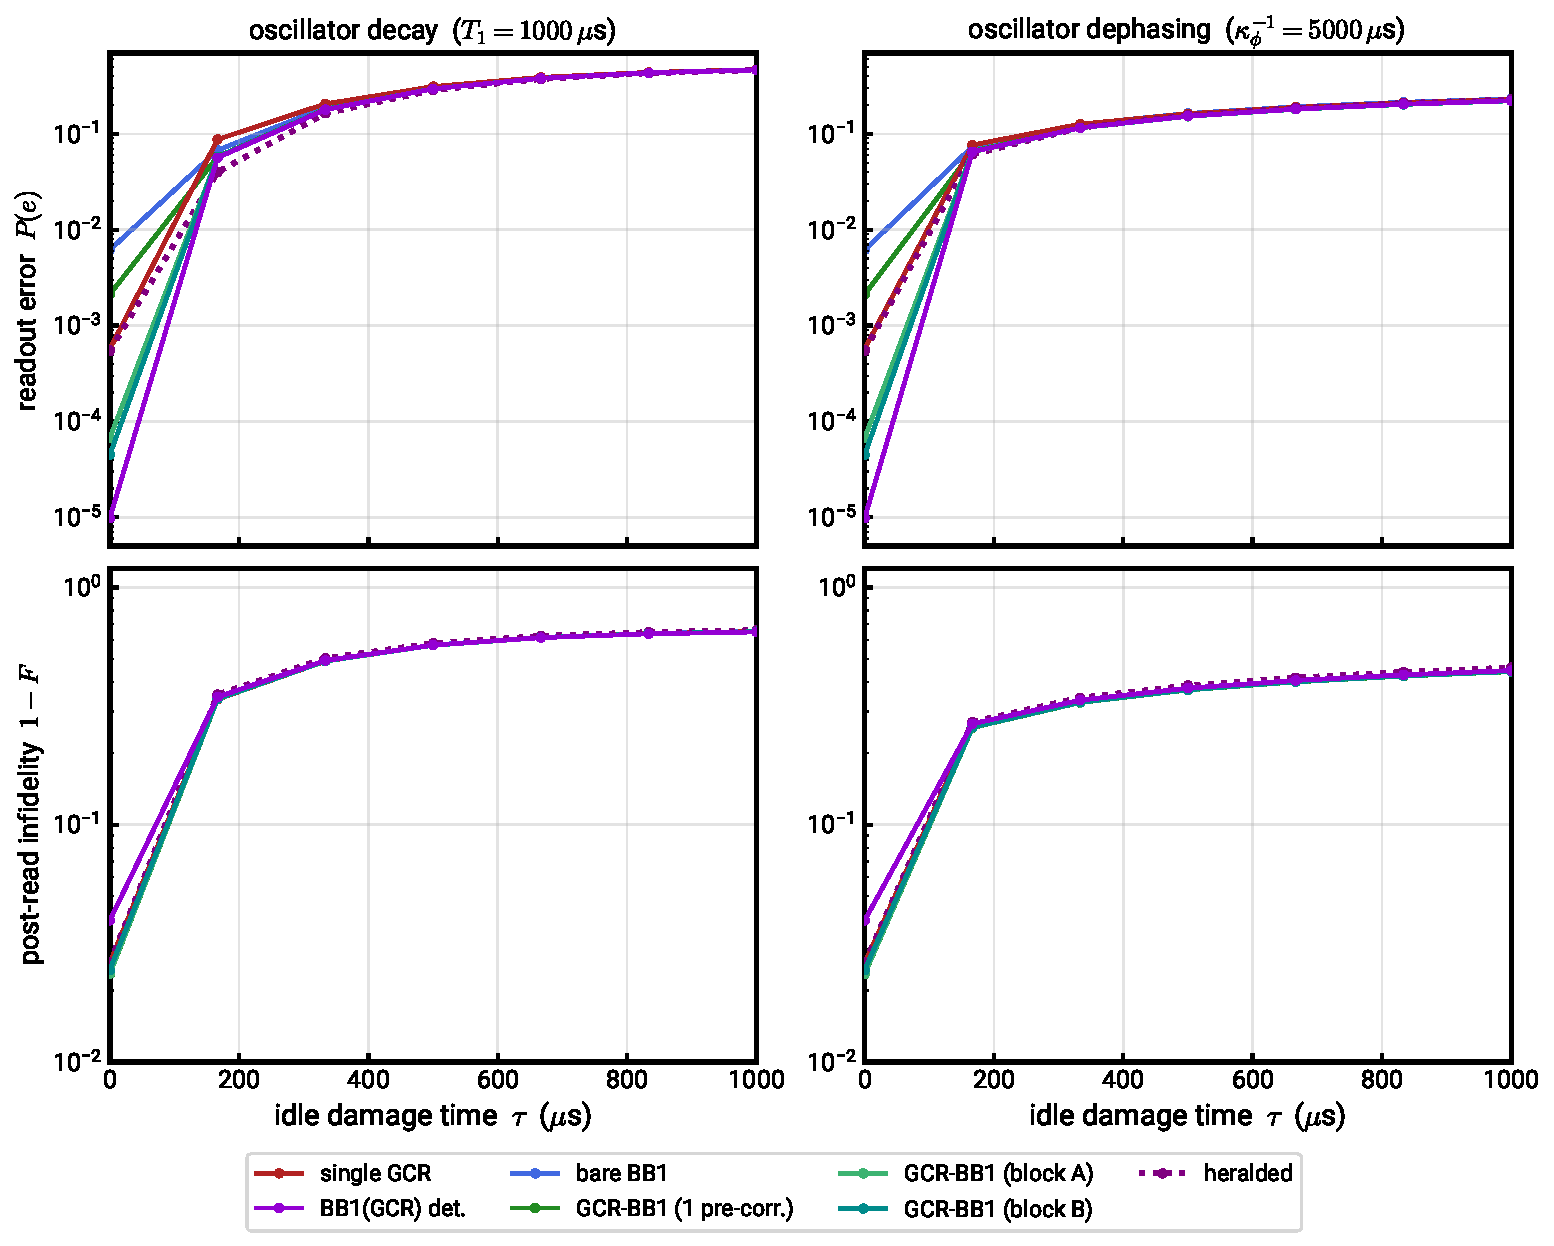
\includegraphics[width=0.92\textwidth]{Paper_Figures/damage_readout.pdf}
\caption{\textbf{Reading a pre-damaged codeword.} Undisplaced no-error logical-$0$/$1$ GKP
codewords are idled under a pure oscillator channel for time $\tau$ and then read with
\emph{noiseless} pulses, isolating the effect of input damage from readout-circuit noise.
Columns: oscillator photon loss ($T_1=1000\,\mu$s, left) and oscillator dephasing
($\kappa_\phi^{-1}=5000\,\mu$s, right). Top row: readout error $P(e)$; bottom row: post-read
oscillator infidelity $1-F$ after a single calibrated corrective displacement. Each panel
overlays the seven readout protocols (colors as in Figs.~\ref{fig:paired-readout} and
\ref{fig:paired-infidelity}); curves are averaged over the two codewords. The $\tau=0$ points
reproduce the noiseless operating points of Sec.~\ref{sec:mesolve}; under photon loss the
$>\!100\times$ spread among protocols collapses to within $1\%$ by $\tau=1000\,\mu$s, as the
lattice information leaks out of the input faster than any readout can extract it.}
\label{fig:damage}
\end{figure}

\paragraph{Noise model.} The experiment has two temporally separate stages, and it is important
to keep their noise sources distinct. We prepare the canonical no-error logical-$0$ and
logical-$1$ codewords --- the $\epsilon=0$ finite-energy GKP states of Sec.~\ref{sec:mesolve},
built with envelope $\Delta=0.34$ in an $N_{\mathrm{cav}}=400$ Fock space --- and first
subject the \emph{bare oscillator} to an idle decoherence stage, then read the damaged state
out. During the idle stage the transmon is uncoupled and the system Hamiltonian is set to
zero, so the density matrix evolves under a purely dissipative Lindblad master equation with a
single collapse operator $\hat L$,
\begin{equation}
\dot\rho \;=\; \mathcal{D}[\hat L]\,\rho
  \;\equiv\; \hat L\,\rho\,\hat L^{\dagger} - \tfrac12\bigl\{\hat L^{\dagger}\hat L,\,\rho\bigr\},
\label{eq:damage-lindblad}
\end{equation}
integrated for an idle time $\tau\in[0,1000]\,\mu$s. Because Eq.~\eqref{eq:damage-lindblad} is
time-independent we integrate it in fixed $20\,\mu$s substeps, which bounds the solver's local
error without changing the channel. We compare two channels on a common $\tau$-axis, each taken
as the \emph{only} dissipator so that its effect is seen in isolation:
\begin{itemize}
  \item \emph{oscillator photon loss}, $\hat L=\sqrt{\kappa}\,\hat a$ with
        $\kappa = 1/T_1^{\mathrm{cav}} = 1/1000\,\mu\mathrm{s}^{-1}$ --- the cavity-$T_1$ rate of
        the Sivak \emph{et al.}\ model used throughout this note. Amplitude damping pulls
        amplitude toward the vacuum, so it \emph{contracts and blurs} the quadrature comb that
        carries the logical bit;
  \item \emph{oscillator dephasing}, $\hat L=\sqrt{\kappa_\phi}\,\hat a^{\dagger}\hat a$ with
        $\kappa_\phi = 1/5000\,\mu\mathrm{s}^{-1}$. The photon-number operator $\hat a^\dagger\hat a$
        commutes with energy, so this channel \emph{smears the comb in phase} while leaving the
        lattice spacing --- and hence the mean photon number --- intact.
\end{itemize}
The Sivak model specifies no intrinsic cavity dephasing, so $\kappa_\phi$ has no hardware
calibration; we deliberately set it a factor of five slower than photon loss and treat the
dephasing column as a \emph{qualitative} comparison of channel character, not a device
prediction. After the idle stage the damaged oscillator is read out by each protocol with
\emph{noiseless} pulses --- the readout circuit itself accrues no decoherence --- so that every
residual error is attributable to the pre-existing input damage alone. This cleanly separates
the input-damage axis studied here from the readout-circuit-noise axis of
Sec.~\ref{sec:mesolve}, whose complementary limit was a pristine input read by noisy pulses.
Figure~\ref{fig:damage} tracks the readout error $P(e)$ and the post-read oscillator infidelity
$1-F$ (after the same single calibrated corrective displacement of Sec.~\ref{sec:mesolve})
against $\tau$, averaged over the two codewords, which are symmetric under both channels.

The dominant message is a \emph{collapse of the protocol hierarchy}. At $\tau=0$ the seven
curves reproduce their noiseless operating points, spanning more than two orders of
magnitude --- from BB1(GCR) and the two blocks at $\sim\!10^{-5}$--$10^{-4}$, up through single
GCR ($6\times10^{-4}$), GCR-BB1 ($2.1\times10^{-3}$), to bare BB1 ($6.1\times10^{-3}$). Idle
photon loss erases this separation almost immediately: the spread is already inside a factor of
$\sim\!2$ by $\tau\approx170\,\mu$s (a sixth of the oscillator $T_1$), inside $10\%$ by
$\tau\approx500\,\mu$s, and by $\tau=1000\,\mu$s all seven agree to within $1\%$, clustered at
$P(e)\approx0.46$ --- just short of the $P(e)=\tfrac12$ random-guess limit. The reason is
physical: the logical bit is carried by the position-quadrature \emph{comb}, and photon loss
contracts and blurs that comb before any pulse acts. Once the lattice information has leaked out
of the input, no readout can recover it, and the choice of correction gadget becomes
irrelevant. Readout engineering buys accuracy only in the regime where the stored state is
still intact.

Dephasing is far gentler at these rates: it smears the comb in phase without contracting the
lattice, and at $\kappa_\phi=1/5000\,\mu\mathrm{s}^{-1}$ the error climbs only to
$P(e)\approx0.22$ by $\tau=1000\,\mu$s, with the hierarchy again collapsing --- the seven
protocols lie within $5\%$ of one another past $\tau\approx330\,\mu$s.

A subtler trend inverts the verdict of Sec.~\ref{sec:mesolve}. There, single GCR was the most
accurate readout because its short circuit accrued the least decoherence. Here, against a
\emph{pre-damaged} input, single GCR is instead the \emph{least} tolerant at intermediate
damage: at $\tau\approx170\,\mu$s it reads at $P(e)=0.087$ (photon loss) and $0.076$
(dephasing), while every BB1-structured scheme sits at $0.040$--$0.068$ and $0.061$--$0.074$
respectively. A single correction gives the narrowest correctable region, so a partially-decayed
input spills past it fastest; the multi-correction schemes, whose entire purpose is to widen
that region, absorb more of the damage-induced spread and degrade more gracefully. The effect
is modest and vanishes once the damage is severe, but it is the mirror image of the
readout-noise story: single GCR wins when the bottleneck is the readout \emph{circuit}, while
the correction-heavy schemes edge ahead when the bottleneck is a \emph{damaged input}.

The post-read oscillator infidelity tells the same story from the state's side, only more
starkly. At $\tau=0$ it reproduces the readout-only floors of Sec.~\ref{sec:mesolve}'s fidelity
table --- $1-F\approx0.023$ for GCR-BB1 and the blocks, rising to $0.040$ for the interleaved
BB1(GCR), the same modest ordering set by the single calibrated corrective displacement. Under
idle damage it climbs monotonically: photon loss drives it to $1-F\approx0.65$ by
$\tau=1000\,\mu$s, dephasing only to $\approx0.44$, again the decay-dominates-dephasing
hierarchy. But the protocol spread here is even tighter than for the readout bit --- the seven
schemes stay within $\lesssim0.016$ of one another at \emph{every} damage time, so the surviving
oscillator overlap is set almost entirely by the input damage and barely at all by which readout
was applied. The one qualitative wrinkle inverts the $P(e)$ ranking once more: the heralded
protocol, the most accurate on the readout bit, leaves the \emph{least} faithful oscillator
state (by $\sim\!0.01$), because its mid-circuit projections perturb the surviving comb slightly
more than the purely-unitary schemes --- heralding optimizes the logical readout, not the state
it leaves behind.

\paragraph{Both hazards at once.} The noiseless-readout panels isolate input damage, but a real
device suffers both hazards together: the stored codeword decays \emph{and} the pulses that read
it are themselves noisy. Figure~\ref{fig:damage-noisy} repeats the damage sweep with the readout
circuit now running under each of the five noise conditions of Sec.~\ref{sec:mesolve}
(all channels, transmon decay, transmon dephasing, oscillator decay, oscillator dephasing),
so that the two axes act simultaneously. The result sharpens rather than softens the verdict.

\begin{figure}[tbp]
\centering
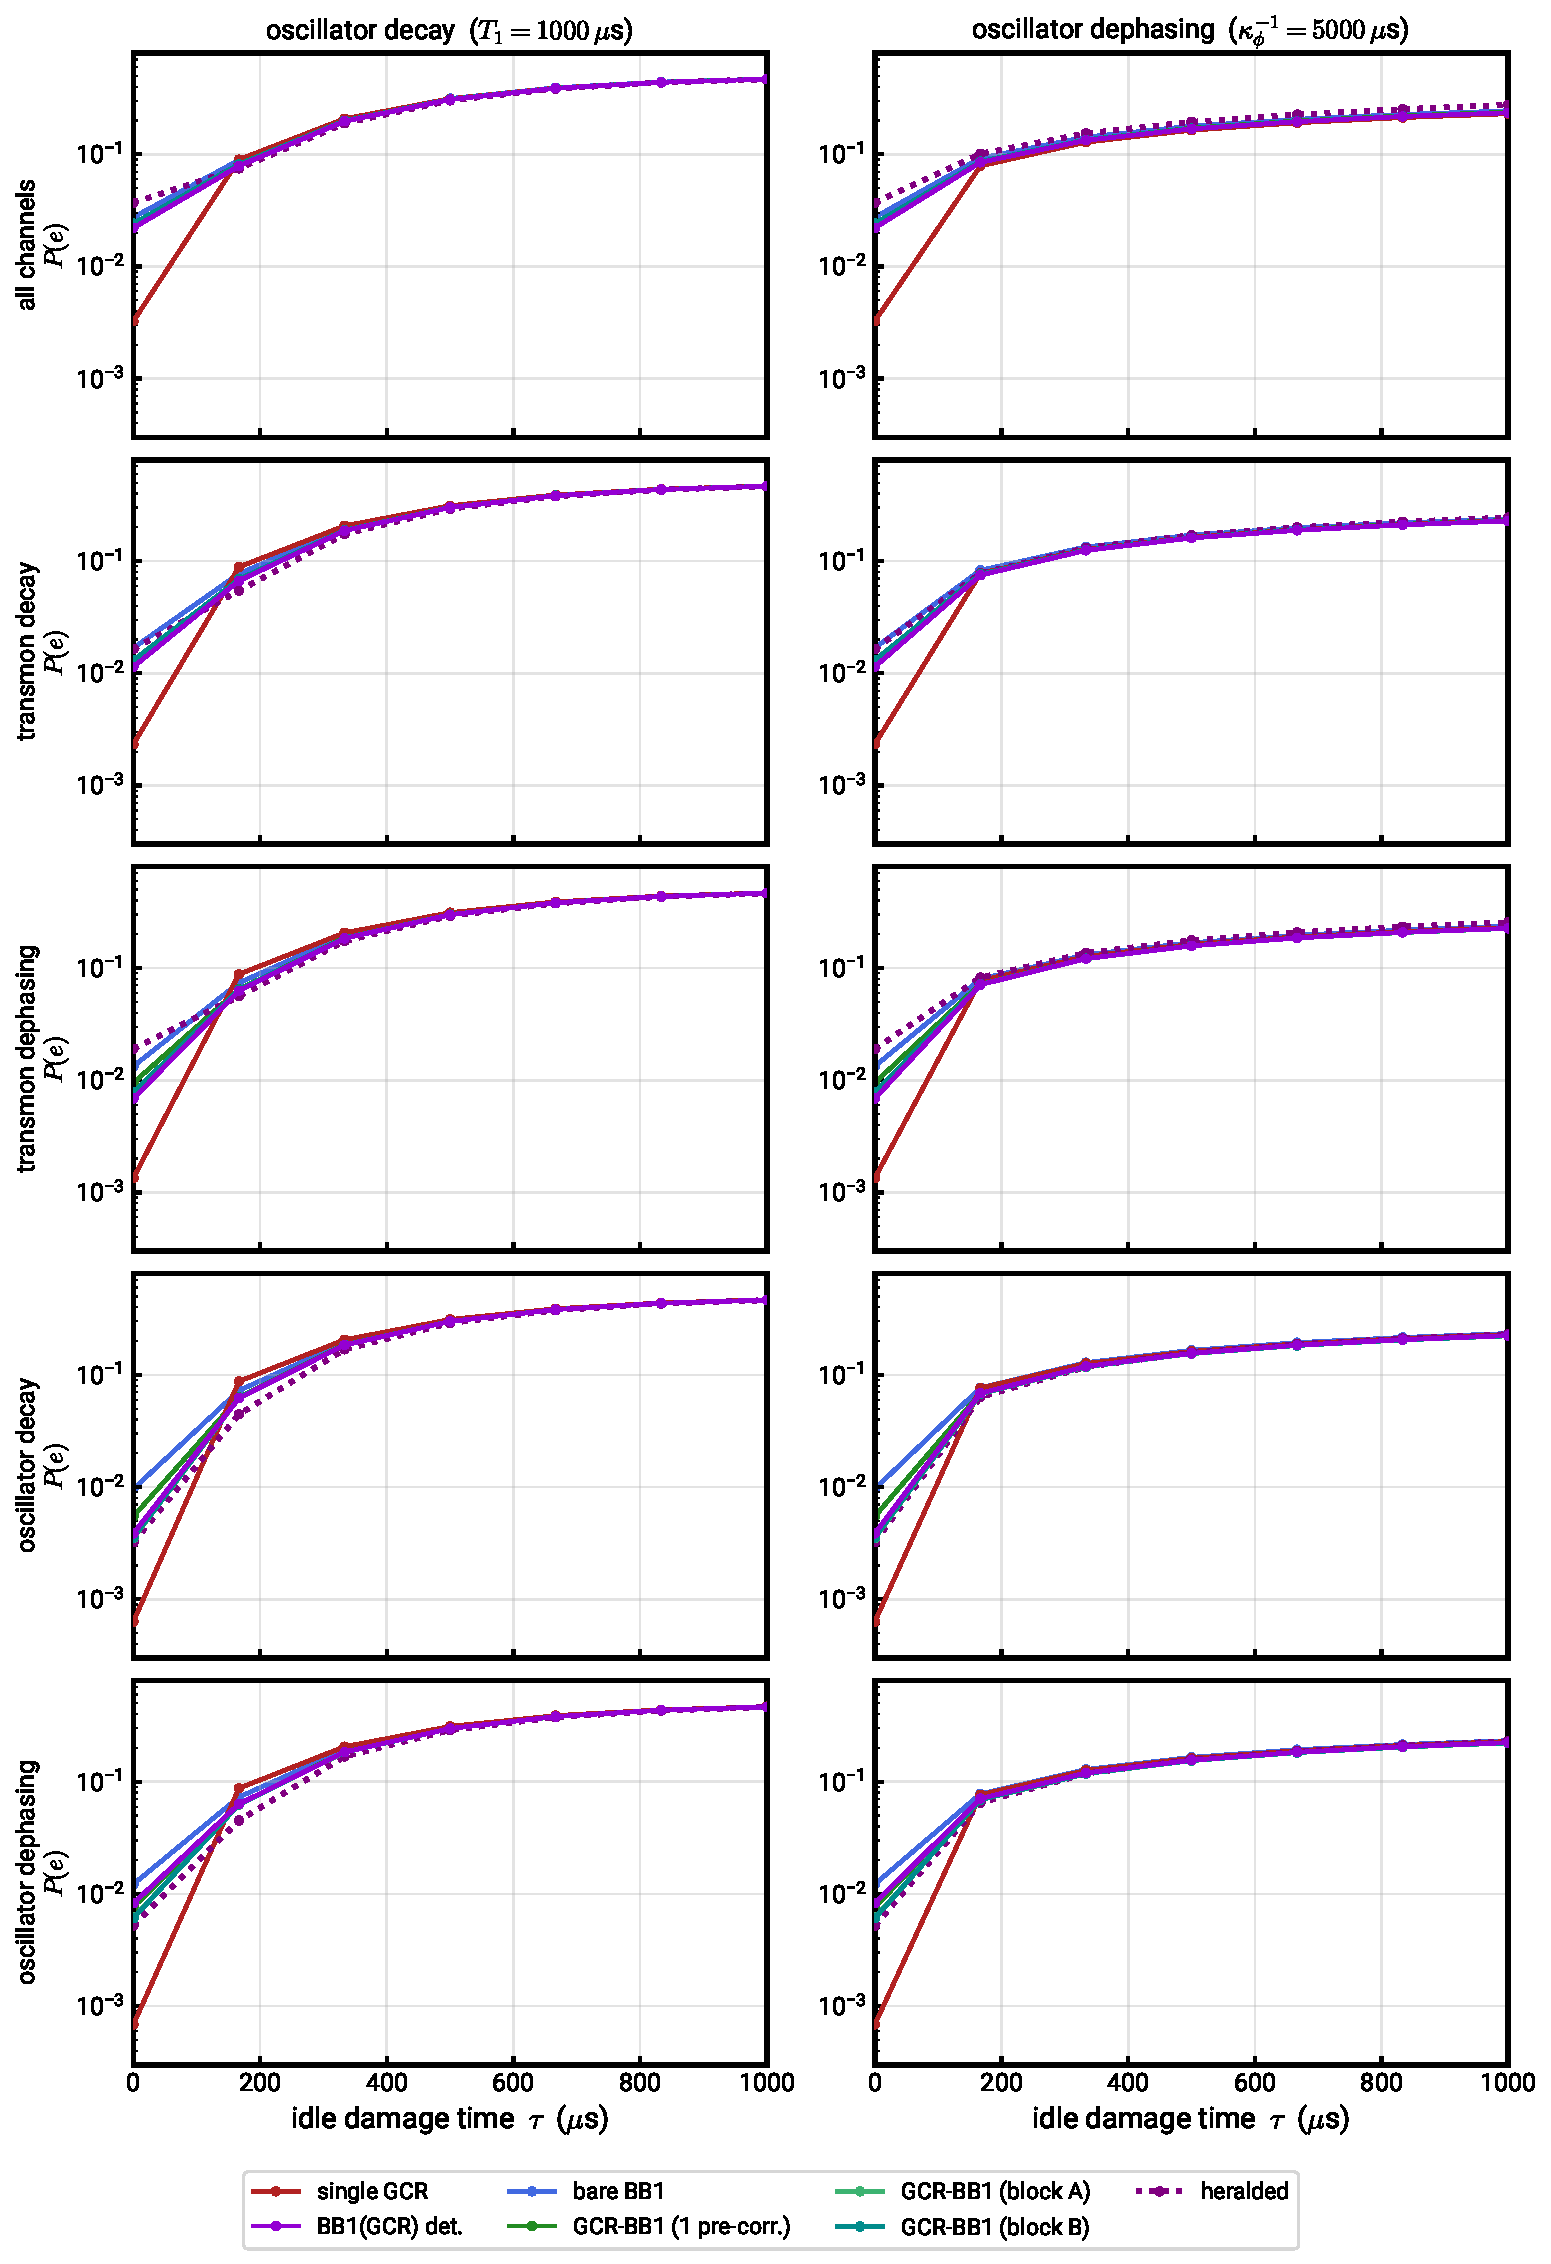
\includegraphics[width=0.92\textwidth]{Paper_Figures/damage_readout_noisy.pdf}
\caption{\textbf{Reading a pre-damaged codeword with \emph{noisy} pulses.} As
Fig.~\ref{fig:damage}, but the readout circuit now accrues decoherence under each of the five
noise conditions of Sec.~\ref{sec:mesolve} (rows), for the two idle-damage channels (columns:
oscillator photon loss, left; oscillator dephasing, right). Curves are the readout error $P(e)$
for the seven protocols, averaged over the two codewords. Readout-circuit noise lifts the
$\tau=0$ floors and \emph{inverts} the protocol ranking there --- the noiseless-best interleaved
BB1(GCR) is now among the worst, single GCR the best --- but the large-$\tau$ tail is set almost
entirely by the input damage and is essentially independent of the readout condition.}
\label{fig:damage-noisy}
\end{figure}

Readout-circuit noise reshuffles the $\tau=0$ operating points and \emph{inverts} the noiseless
ranking, exactly as Sec.~\ref{sec:mesolve} predicts. Under the all-channels condition the
interleaved BB1(GCR), which reads at $\sim\!10^{-5}$ with noiseless pulses, is lifted to
$P(e)=2.2\times10^{-2}$ --- now among the \emph{worst} protocols --- while single GCR, whose
short circuit accrues the least decoherence, sits lowest at $3.3\times10^{-3}$, and the heralded
scheme trails at $3.7\times10^{-2}$. The correction-heavy circuits pay for their length in
readout noise: the very structure that buys a near-Helstrom noiseless floor becomes a liability
the moment the pulses are lossy. Weakening the readout channel (transmon dephasing, oscillator
dephasing) lowers these floors uniformly but preserves the ordering, with single GCR always the
most accurate read at $\tau=0$.

The interplay of the two axes produces a clean \emph{crossover}. Single GCR is the best readout
at $\tau=0$ but the least tolerant of a decayed input; as damage accumulates its curve rises
through the pack, and by $\tau\approx167\,\mu$s under all-channels readout it is the \emph{worst}
of the seven ($P(e)=0.090$, against $0.075$ for the correction-heavy schemes) --- the mirror
image of its $\tau=0$ lead. This is the two sections meeting in a single figure: single GCR wins
when the bottleneck is the readout \emph{circuit} and loses when it is a \emph{damaged input},
and the changeover sits near $\tau\sim150\,\mu$s for these rates. Past that point every protocol
collapses together exactly as in the noiseless case.

Most telling is what the readout noise does \emph{not} change. At $\tau=1000\,\mu$s all seven
protocols cluster at $P(e)=0.467$ under photon loss and $\approx0.23$ under dephasing --- and
these tail values are identical, to better than $10^{-3}$, across \emph{all six} readout
conditions including the noiseless one. Once the input is destroyed, whatever noise the readout
pulses add is a negligible perturbation on top of information that has already leaked out of the
oscillator. The post-read oscillator infidelity (Fig.~\ref{fig:damage-noisy-infid}) tells the
same story from the state's side: the $\tau=0$ floors are lifted to
$1\text{--}7\times10^{-2}$ depending on the readout condition --- the interleaved BB1(GCR) again
paying the most, up to $7.1\times10^{-2}$ under oscillator-dephasing readout --- yet the tails
converge to $1-F\approx0.65$ (loss) and $\approx0.44$ (dephasing) essentially independent of
which pulses were used. Adding realistic readout noise therefore does not rescue the hierarchy
--- it only confirms that beyond a modest damage threshold the outcome is a \emph{memory} failure
that no readout, noisy or clean, can undo.

\begin{figure}[tbp]
\centering
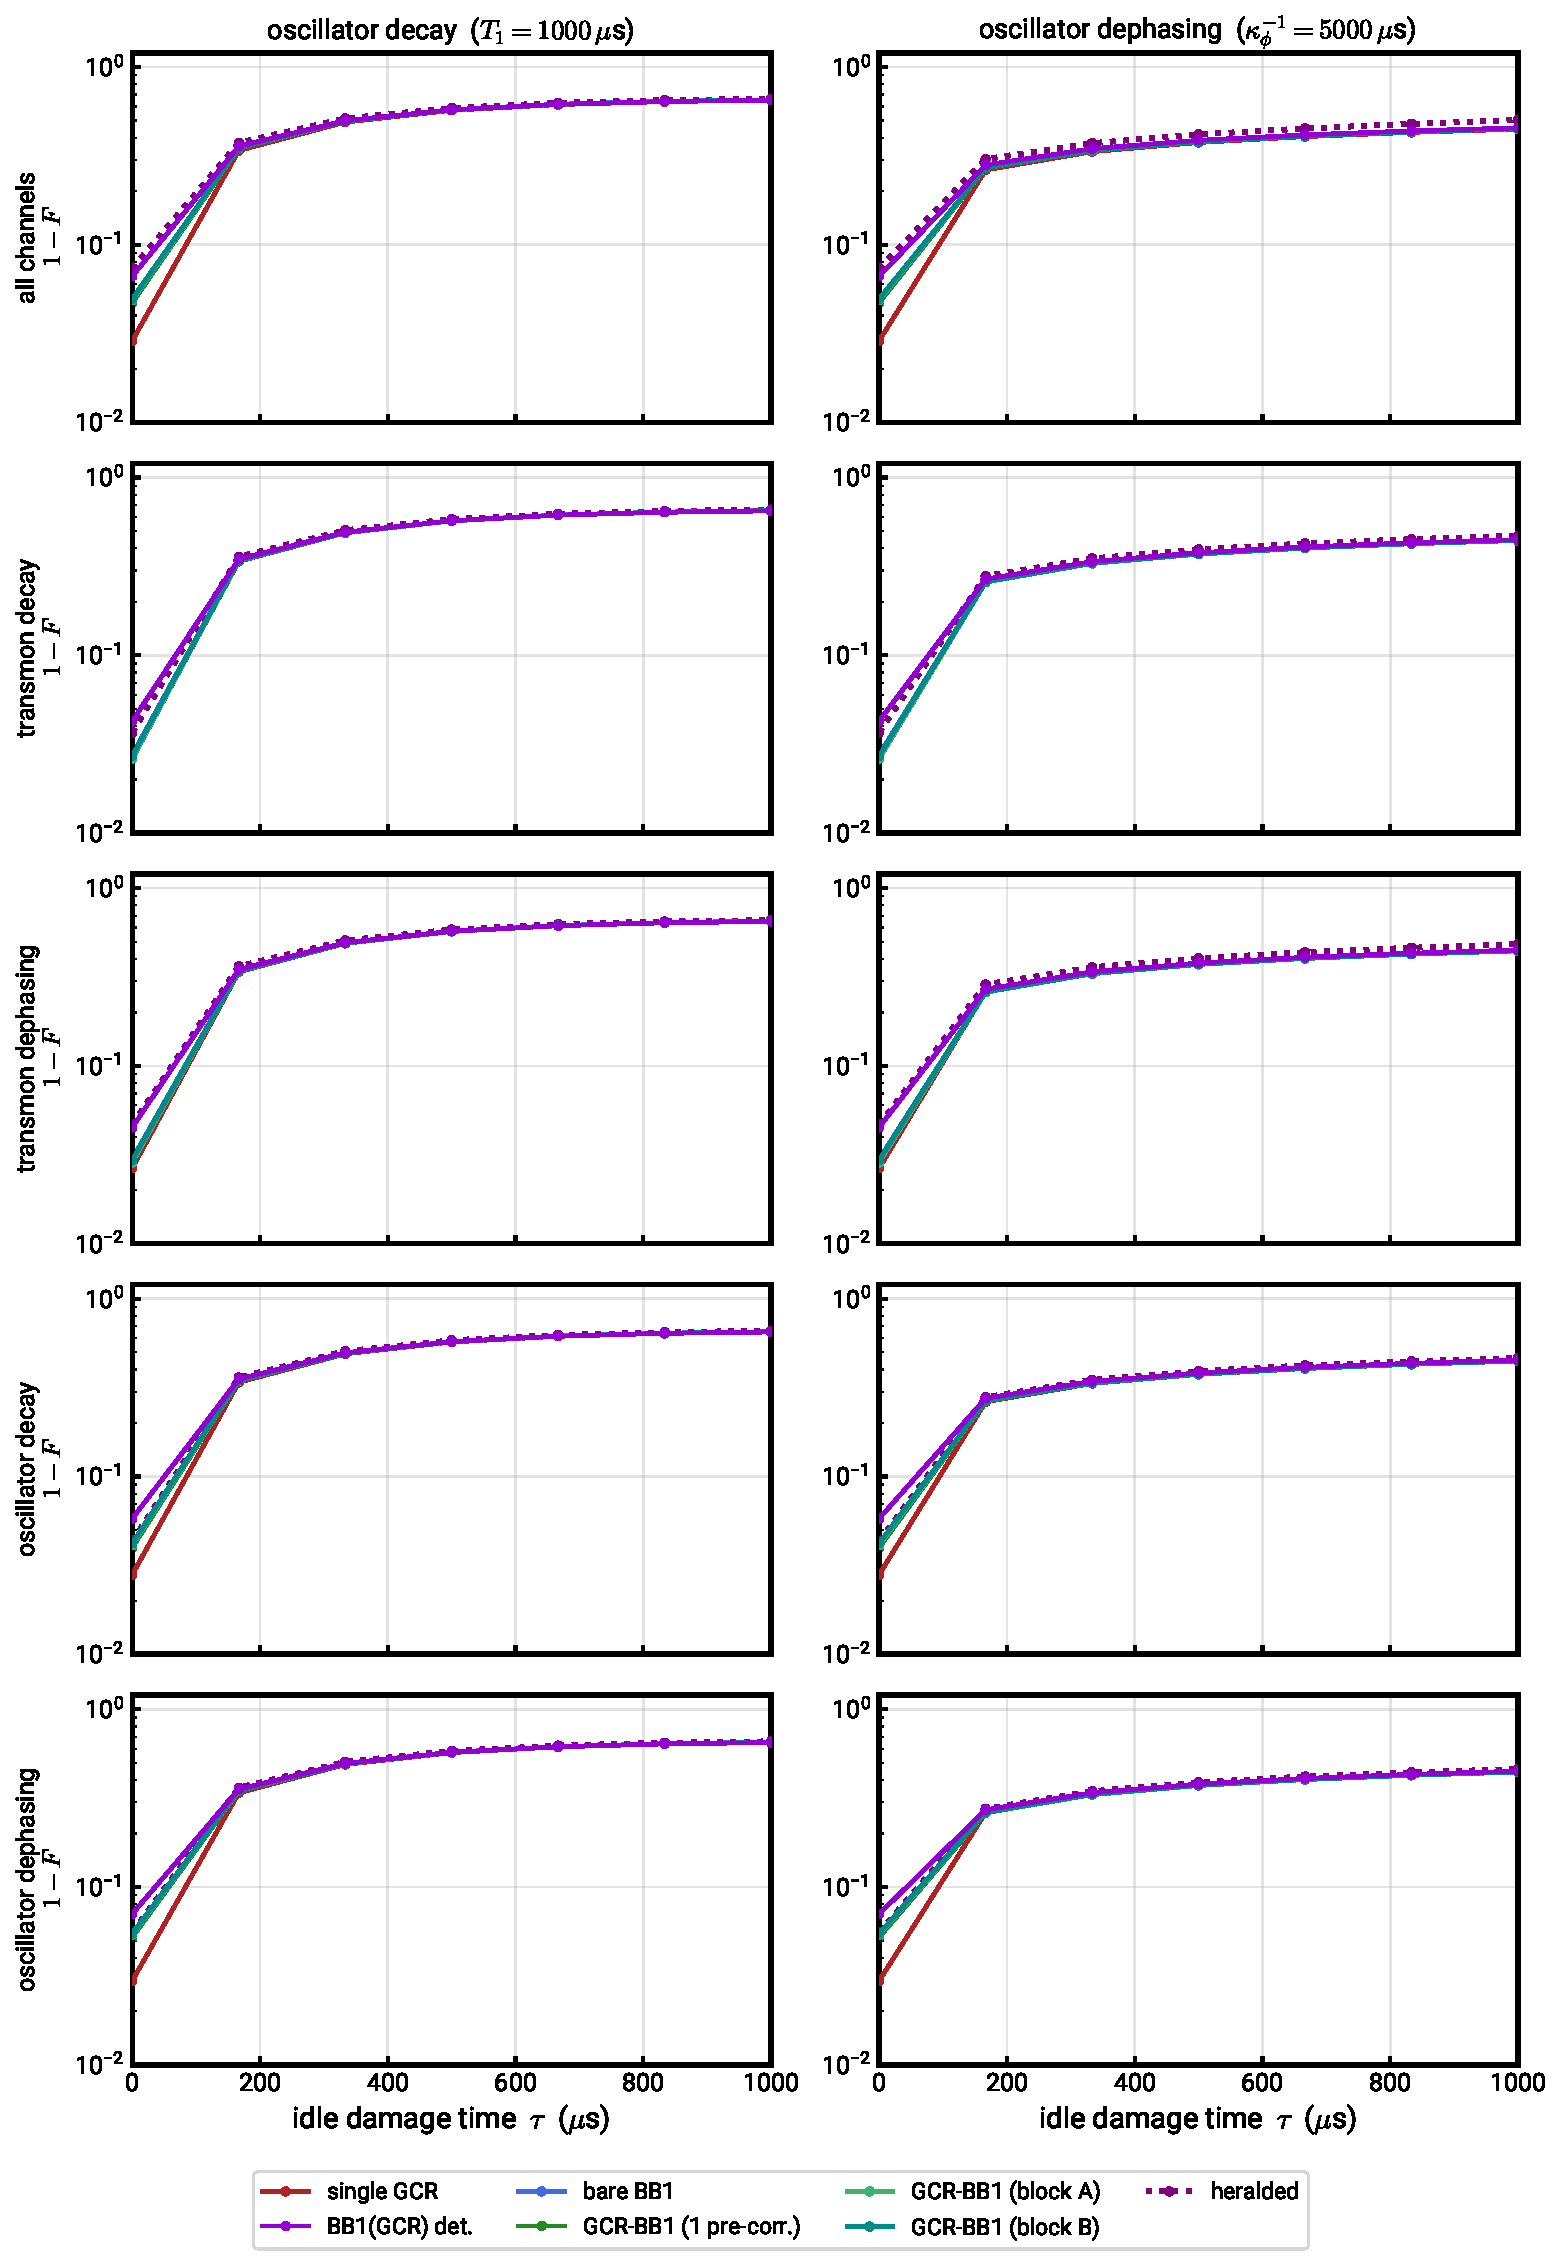
\includegraphics[width=0.92\textwidth]{Paper_Figures/damage_readout_noisy_infid.pdf}
\caption{\textbf{Post-read oscillator infidelity with noisy pulses.} Companion to
Fig.~\ref{fig:damage-noisy} on the identical grid: post-read oscillator infidelity $1-F$ (after
the single calibrated corrective displacement) for the five readout-noise conditions (rows) and
the two idle-damage channels (columns), seven protocols overlaid. As for the readout bit, the
readout condition sets only the lightly-damaged floors; the heavily-damaged tails
($1-F\approx0.65$ under photon loss, $\approx0.44$ under dephasing) are fixed by the input damage
and are common to all conditions.}
\label{fig:damage-noisy-infid}
\end{figure}

Together with Sec.~\ref{sec:mesolve}, this bounds the operational value of the whole
construction. The elaborate corrections earn their keep against readout-circuit noise, and buy
a modest graceful-degradation margin against a lightly-damaged input; but a heavily-damaged
codeword is a \emph{memory} failure, not a readout failure, and is beyond the reach of any
readout. The remedy there is a better oscillator or more frequent stabilization --- not a
longer pulse train.

\FloatBarrier
\section{Reading an actively stabilized codeword: noisy SBS rounds before readout}\label{sec:sbs}

Section~\ref{sec:damage} let the codeword idle passively. A real logical memory does the
opposite: it is \emph{actively stabilized}, its lattice periodically re-sharpened by an
error-correction protocol that itself runs on the same imperfect hardware. The canonical GKP
stabilizer is the small--big--small (SBS) round of Royer \emph{et al.}\ and
Campagne-Ibarcq \emph{et al.}, realized on the Sivak \emph{et al.}\ device: a sequence of
conditional displacements interleaved with ancilla rotations that pumps entropy out of the
oscillator and pushes the state back toward the code manifold. But each round is a finite-duration
circuit coupling the oscillator to a lossy ancilla, so stabilization is a double-edged tool ---
it removes lattice error while injecting fresh decoherence. We ask how this trade-off interacts
with the readout: after $m$ rounds of \emph{noisy} SBS, how faithfully does each of the seven
protocols read the stabilized codeword, and how does that degrade as the rounds accumulate?

\paragraph{Model.} We use the authentic SBS protocol of the Sivak \emph{et al.}\
device --- a $\sigma_z$-conditioned time evolution under the marker Hamiltonians
$\hat H_x=\hat\sigma_z\otimes a_1\hat x$ and $\hat H_p=-\hat\sigma_z\otimes a_1\hat p$, with an
$R_x(\pi/2)$ rotation conjugating the big step, acting on a finite-energy \emph{binomial} GKP
codeword ($\Delta=0.34$, $N_{\mathrm{cav}}=200$). The fresh $m=0$ codeword is the fixed point of
noiseless cooling: we run the stabilizer forward from vacuum for twenty rounds to obtain the
stabilized logical-$0$ state $G_{\mathrm{SBS},0}$, and take that as the input to the experiment.
A single SBS round of this protocol exchanges the two logical branches --- it is a stable
two-cycle, $G_{\mathrm{SBS},0}\!\leftrightarrow\!G_{\mathrm{SBS},1}$, with the fidelity returning
to $\gtrsim0.98$ after every second round --- so we sample an even number of rounds
$m\in\{0,2,4,6,8,10\}$, for which the encoding always returns to logical $0$ while having absorbed
the decoherence of $m$ physical stabilization circuits.\footnote{This parity exchange is a feature
of a single SBS round, not a defect: it is why the cooling trajectory alternates between the
$\mu=0$- and $\mu=1$-like states on consecutive iterations. Odd $m$ would simply read the
logical-$1$ branch of the same data.}

Noise enters the SBS rounds through the same collapse operators used throughout this note. During
the marker evolutions the master equation carries, according to the condition under test, transmon
decay $\sqrt{\gamma}\,\hat\sigma_-$ ($\gamma=1/200\,\mu\mathrm{s}^{-1}$), transmon dephasing
$\sqrt{\gamma_\phi/2}\,\hat\sigma_z$ ($\gamma_\phi=1/200\,\mu\mathrm{s}^{-1}$), oscillator photon
loss $\sqrt{\kappa}\,\hat a$ ($\kappa=1/1000\,\mu\mathrm{s}^{-1}$), or oscillator dephasing
$\sqrt{\kappa_\phi}\,\hat a^\dagger\hat a$ ($\kappa_\phi=1/5000\,\mu\mathrm{s}^{-1}$, the same
qualitative rate as in Sec.~\ref{sec:damage}). We run five separate stabilization experiments, one
per SBS-noise condition: \emph{all channels} together (transmon decay $+$ transmon dephasing $+$
oscillator loss), and each of transmon decay, transmon dephasing, oscillator decay, and oscillator
dephasing in isolation. In every experiment the stabilized state at each $m$ is then read out under
all six readout-circuit conditions of Sec.~\ref{sec:mesolve} --- noiseless, all channels, transmon
decay, transmon dephasing, oscillator decay, oscillator dephasing --- so that the SBS-noise axis
and the readout-noise axis are cleanly separated. As before we report the readout error $P(e)$ and
the post-read oscillator infidelity $1-F$ after the single calibrated corrective displacement,
against the pristine $m=0$ codeword; the analysis is for logical $0$.

\paragraph{A note on the vertical scale.} Because a genuine, non-collapsing SBS stabilizer is
available only in the device's native \emph{binomial}-GKP, $i=2$ quadrature convention, this
section uses that codeword rather than the Gaussian-comb encoding of
Secs.~\ref{sec:mesolve}--\ref{sec:damage}. The stabilized codeword is correspondingly softer than
the idealized comb --- even the freshly-cooled $m=0$ state reads at $P(e)\approx0.08$ under
noiseless pulses, the validated operating point of this SBS stabilizer, rather than the
$\lesssim10^{-3}$ floors of Sec.~\ref{sec:mesolve}. The comparison of interest here is therefore
\emph{relative}: how each protocol and each noise channel move the operating point as the rounds
accumulate, not the absolute floor, which is set by the encoding rather than the readout gadget.

\paragraph{Heralding does not transfer to the stabilized codeword.} One protocol must be set
aside at the outset. Unlike the six deterministic protocols --- whose corrections are conditional
\emph{displacements} that act relative to the state and therefore inherit whatever lattice the
codeword carries --- the heralded scheme relies on a fixed, non-covariant momentum \emph{filter}
whose geometry is pinned to the Gaussian-comb lattice of Secs.~\ref{sec:mesolve}--\ref{sec:damage}.
On the binomial-GKP fixed point of this SBS stabilizer, that filter is mis-registered: a
scan of the input displacement over a full two-cell window fails to bring the heralded readout below
$P(e)\approx0.47$ anywhere on the real axis, and momentum-axis displacements drive the
post-selection norm through zero (the heralding branch is rejected) rather than recovering it. In
other words, the heralded gadget would have to be re-derived from scratch for each encoding's
lattice; a rigid recalibration cannot rescue it. We therefore report the \emph{six deterministic}
protocols here and note only that the heralded scheme, alone among the seven, is not portable across
the encoding change --- a concrete cost of building readout around a lattice-specific measurement.

\paragraph{Noisy stabilization degrades readout slowly, and the ancilla is the culprit.}
Figure~\ref{fig:sbs} isolates the stabilization noise by reading every state under noiseless
pulses. All six protocols start from the same freshly-cooled floor, $P(e)\in[0.079,0.085]$ at
$m=0$, and rise gently and near-linearly as noisy rounds accumulate. The \emph{rate} of that rise
is set almost entirely by which channel is active during the SBS circuit, and the ordering is
sharp: transmon decay is by far the most damaging ($P(e)$ climbs $0.079\!\to\!0.097$ over ten
rounds), and the all-channels case tracks it almost exactly ($0.079\!\to\!0.098$), while
oscillator dephasing ($0.079\!\to\!0.086$), oscillator decay ($0.079\!\to\!0.083$) and transmon
dephasing ($0.079\!\to\!0.083$) each add only a few $\times10^{-3}$ over the whole sweep. That the
ancilla's $T_1$ dominates --- and that isolated oscillator loss is nearly harmless --- is exactly
what one expects of an actively-pumped stabilizer: the transmon is entangled with the oscillator
throughout each conditional displacement, so its decay corrupts the round it drives, whereas slow
photon loss is continually undone by the very map that injects it. Across the entire sweep the six
protocols stay bunched within a $\lesssim5\times10^{-3}$ band: once the codeword is being actively
stabilized, the choice of readout dressing matters far less than how many noisy rounds it has seen
and through which channel.

\paragraph{Readout noise adds a separable offset, and the shortest circuit wins.}
Figure~\ref{fig:sbs-readout} holds the stabilization at its realistic all-channels setting and
sweeps the readout circuit over its six noise conditions. Adding readout noise leaves the shape of
the $m$-dependence intact and shifts each protocol up by a nearly $m$-independent offset, so the two
noise axes are separable. But the offset is strongly \emph{protocol}-dependent, and it tracks the
\emph{duration} of the readout circuit rather than its correction content: single GCR --- the
shortest deterministic sequence, one pre-correction and one kick --- is almost immune, its $P(e)$
rising by only $+2.5\times10^{-3}$ under all-channels readout, while the five longer circuits are
lifted \emph{together} by $+1.8$ to $+2.0\times10^{-2}$, whether or not they carry detuning
corrections (bare BB1, with none, is lifted as much as the detuning-heavy schemes). Readout noise
therefore does not blur the family uniformly; it drives single GCR clearly below the pack and
widens the protocol band from $\sim6\times10^{-3}$ under noiseless pulses to $\sim2\times10^{-2}$.
The offset again follows the transmon --- all-channels and transmon-decay readout dominate
($\approx1.6$ and $0.9\times10^{-2}$ on average), oscillator decay contributes least
($\lesssim3\times10^{-3}$) --- reproducing the verdict of Sec.~\ref{sec:damage}: under
readout-circuit noise the least-exposed, shortest protocol is the most accurate, and the elaborate
corrections pay for their length.

\begin{figure}[tbp]
\centering
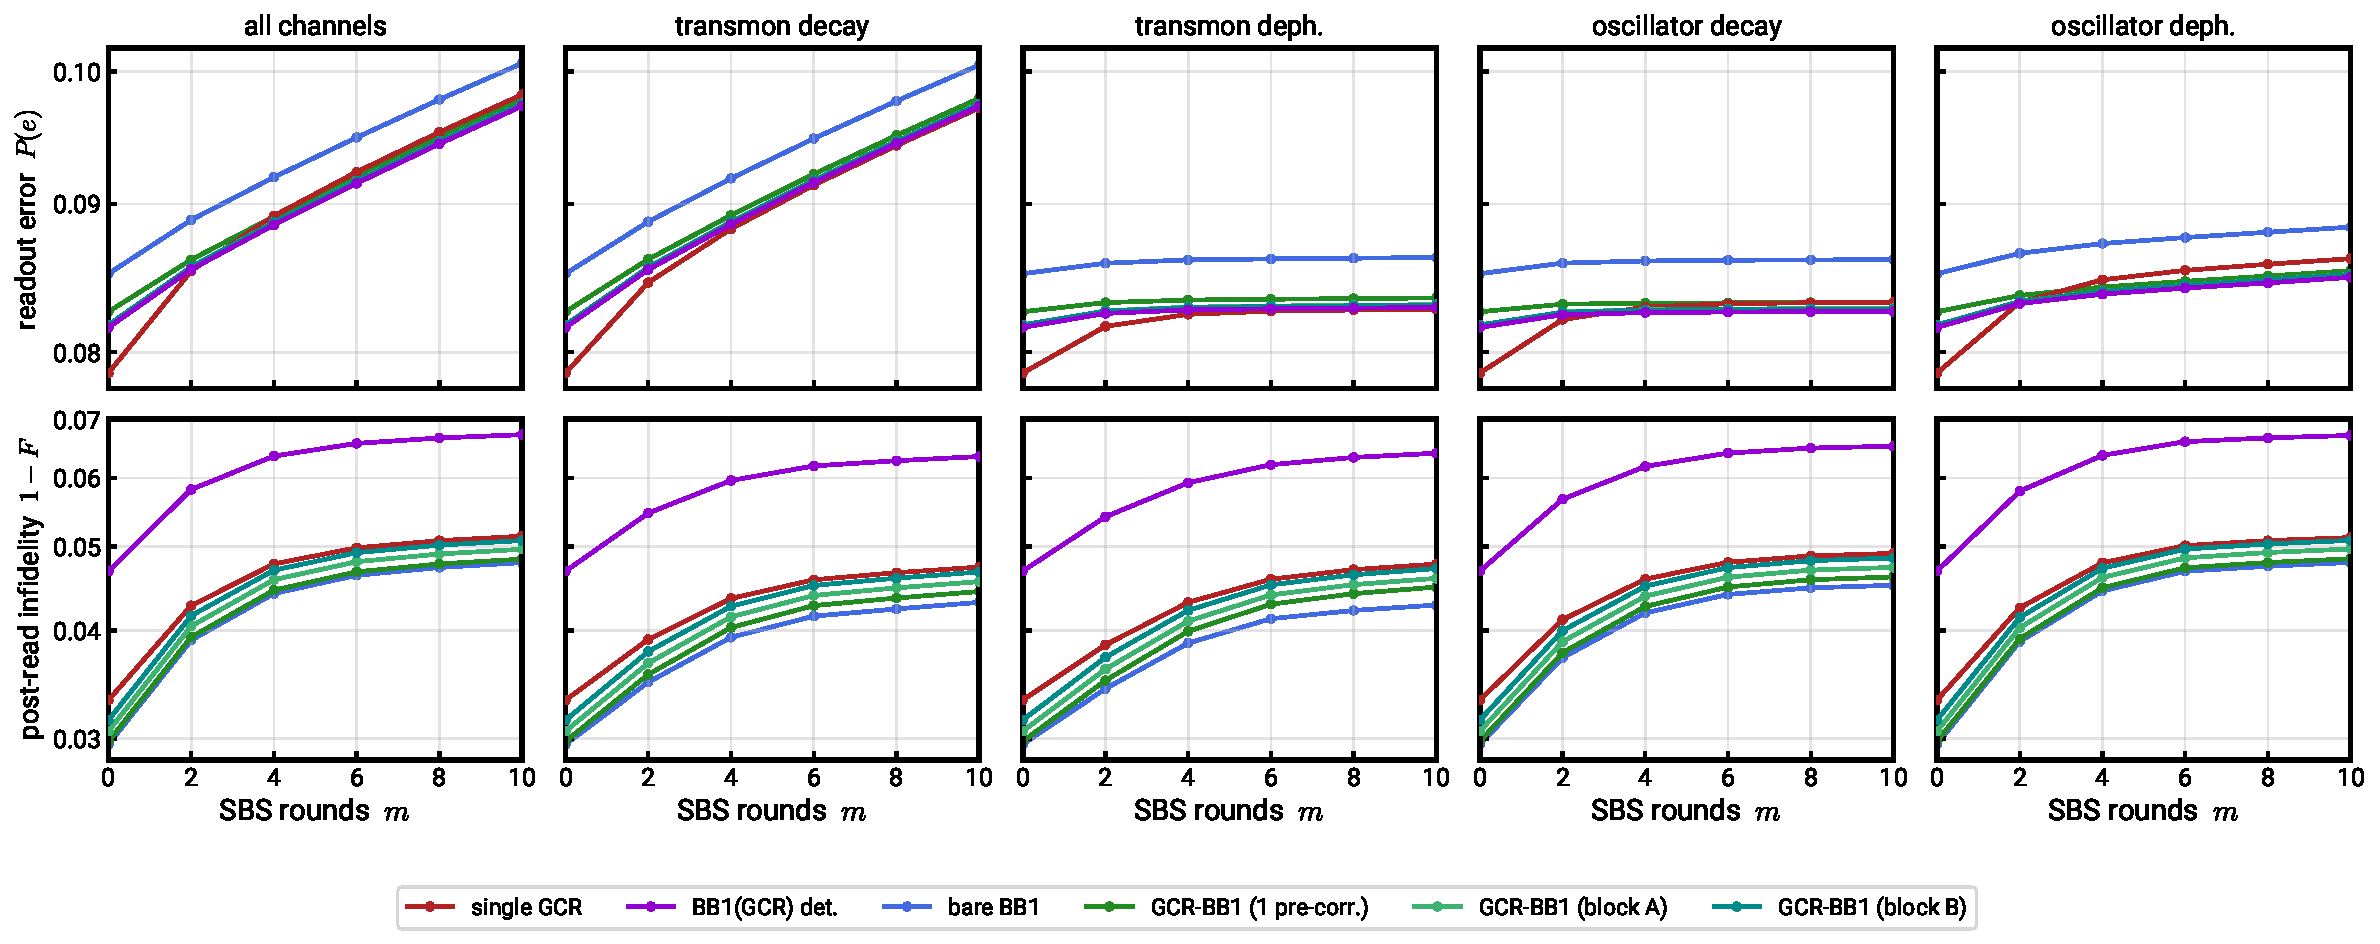
\includegraphics[width=\textwidth]{Paper_Figures/sbs_readout_sweep.pdf}
\caption{Reading an actively-stabilized logical~$0$ after $m$ rounds of \emph{noisy} SBS, under
\emph{noiseless} readout (isolating the stabilization noise). Columns are the five SBS-noise
conditions; top row is the readout error $P(e)$, bottom row the post-read oscillator infidelity
$1-F$; each panel overlays the six deterministic protocols versus the number of rounds $m$ (the
heralded scheme is omitted, see text). Note the logarithmic vertical scale (chosen to expose the
small protocol-to-protocol differences on the high binomial-SBS floor). All protocols share the
freshly-cooled floor at $m=0$ and rise gently; the rise is dominated by transmon decay (and the
all-channels case tracks it), while the oscillator channels and transmon dephasing are far
gentler. On $P(e)$ (top) the six protocols stay bunched within a few~$\times10^{-3}$ throughout;
on $1-F$ (bottom) BB1(GCR) det.\ (purple) separates cleanly as the least-faithful, sitting
$\approx1.4$--$1.6\times10^{-2}$ above the tightly-grouped pack (bare BB1, GCR-BB1 and the two
blocks lowest, single GCR just above them).}
\label{fig:sbs}
\end{figure}

\begin{figure}[tbp]
\centering
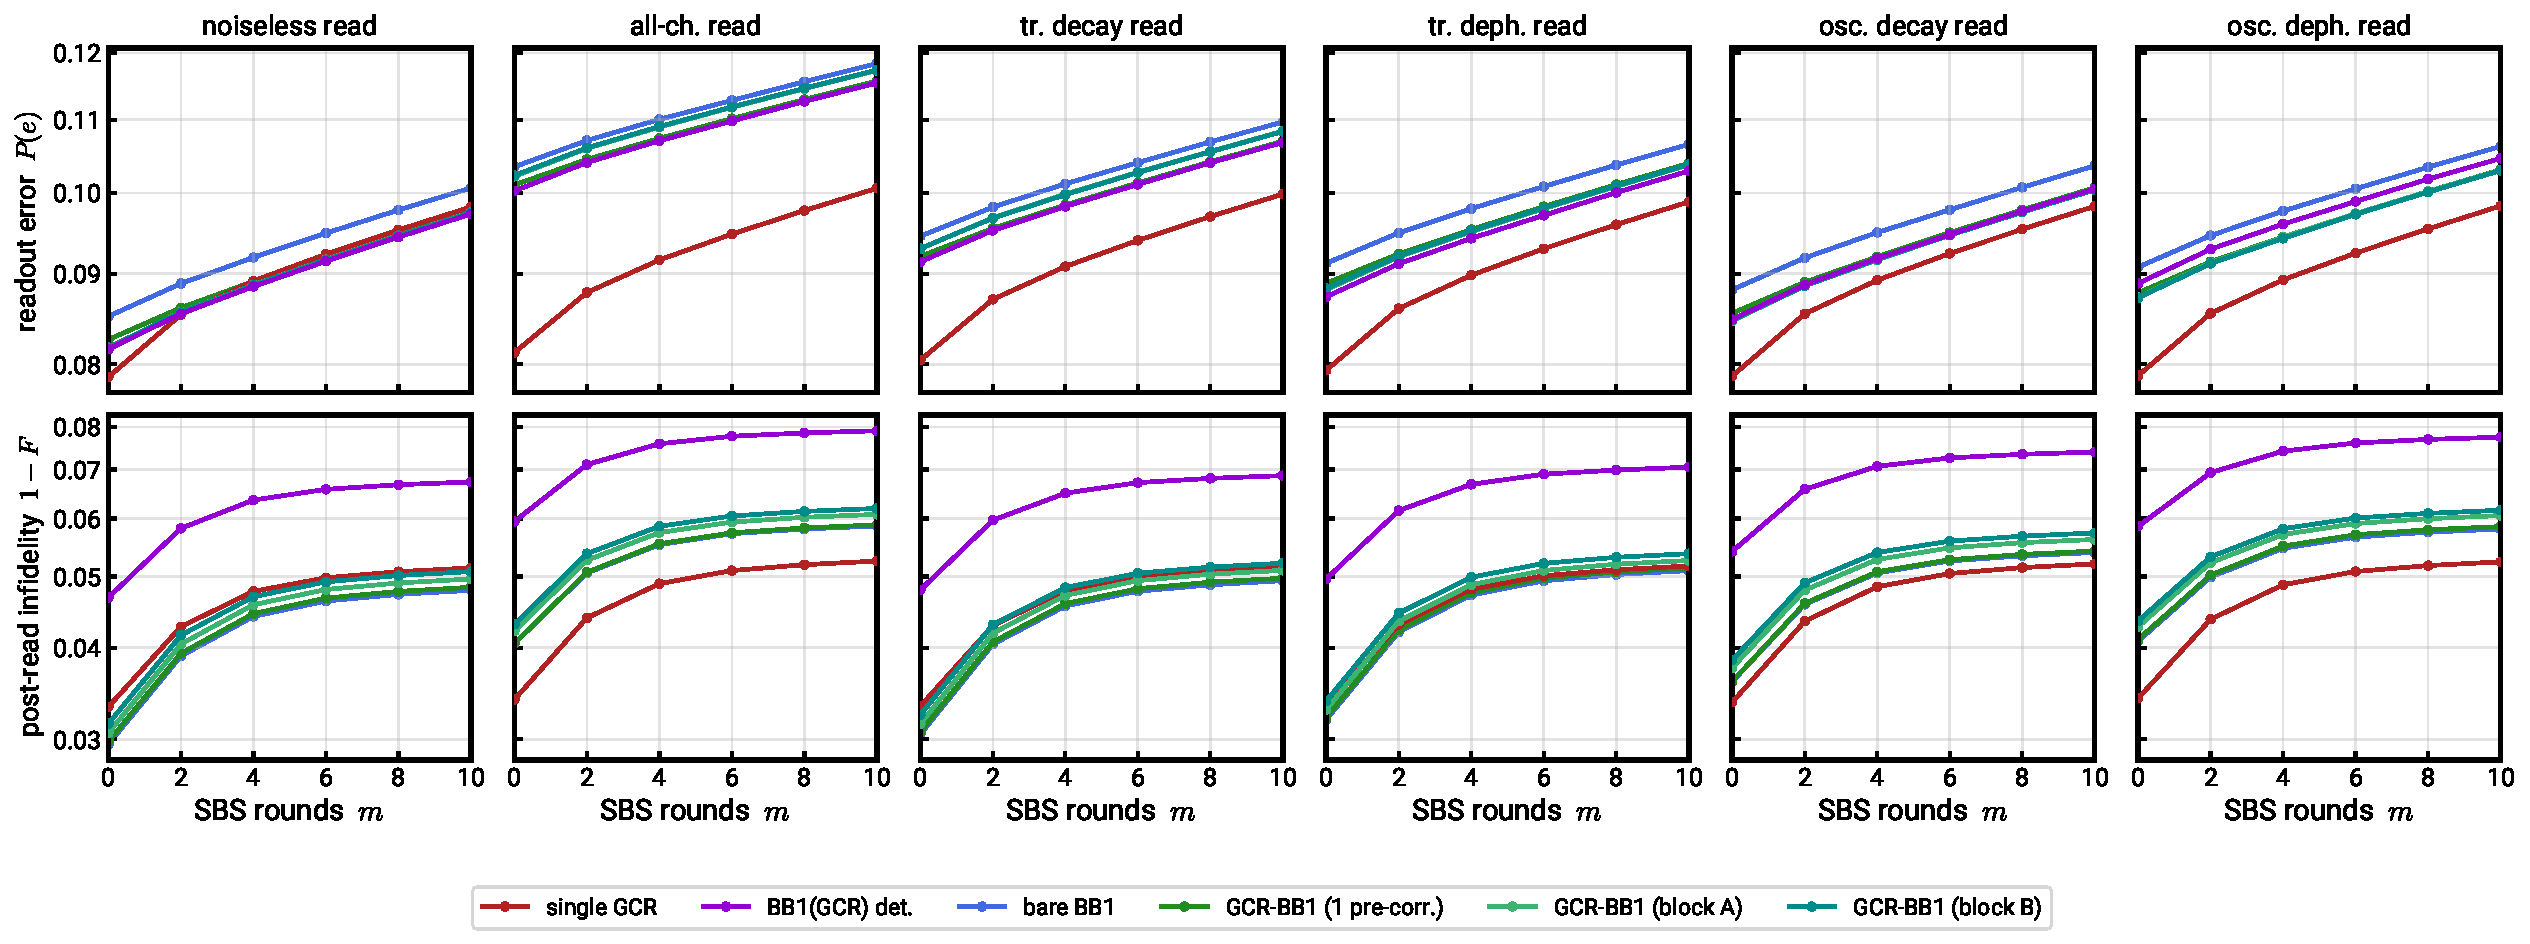
\includegraphics[width=\textwidth]{Paper_Figures/sbs_readout_conds.pdf}
\caption{The same experiment with the SBS stabilization fixed at its realistic all-channels
setting, now sweeping the \emph{readout}-circuit noise across its six conditions (columns). Rows
and curves as in Fig.~\ref{fig:sbs}; logarithmic vertical scale. Readout noise shifts the
$m$-dependence up by a nearly constant, $m$-independent offset --- the two noise axes are separable
--- largest for transmon decay and the all-channels case, smallest for oscillator decay. The offset
tracks circuit \emph{duration}: under all-channels readout the freshly-cooled ($m{=}0$) $P(e)$ rises
by only $+2.5\times10^{-3}$ for single GCR (red) but by $+1.8$ to $+2.0\times10^{-2}$ for the five
longer protocols, so single GCR pulls clearly below the pack (which lifts together regardless of
correction content) --- reproducing the short-circuit-wins verdict of Sec.~\ref{sec:damage}.}
\label{fig:sbs-readout}
\end{figure}

\paragraph{The state's-eye view, and the bottom line.} The oscillator infidelity
(bottom rows of Figs.~\ref{fig:sbs}--\ref{fig:sbs-readout}) tells the same story with one
addition. Starting from $1-F\in[0.030,0.047]$ at $m=0$, the post-read infidelity rises and then
\emph{saturates} beyond $m\approx4$: the noisy stabilizer reaches a fixed point at which entropy
injected per round balances entropy pumped out, so the state stops degrading rather than drifting
without bound. Here the protocol ordering does separate, and it \emph{inverts} between the two
metrics: bare BB1, which carries the \emph{largest} readout error of the six, nonetheless leaves
the \emph{most} faithful oscillator state ($1-F$: $0.030\!\to\!0.048$ over $m=0\!\to\!10$), while the
detuning-heavy BB1(GCR) correction --- among the best at pinning the readout bit --- leaves the
\emph{least} faithful state ($0.047\!\to\!0.067$), a clear $\approx\!1.4$--$1.6\times10^{-2}$ above
the rest of the pack (single GCR $0.033\!\to\!0.051$; GCR-BB1 and the two blocks bunched between bare
BB1 and single GCR). The sharpest single comparison is single GCR versus BB1(GCR), the two protocols
that best pin the bit: on $P(e)$ they are \emph{tied} to within $\sim\!10^{-3}$
($0.079\!\to\!0.098$ vs $0.082\!\to\!0.097$ under noiseless readout), but on the oscillator state
single GCR is better by $\approx\!1.4\times10^{-2}$ at every $m$. So on this soft, actively-stabilized
codeword BB1(GCR) \emph{strictly loses} to single GCR --- its three extra detuning corrections and
three extra kicks buy nothing measurable on the bit while imprinting $\sim\!1.4\times10^{-2}$ more
back-action on the oscillator; the sub-$10^{-3}$ coherent-floor edge that justifies BB1(GCR) on a
pristine comb (Sec.~\ref{sec:mesolve}) is simply below the $\sim\!0.08$ binomial floor here. As in
Sec.~\ref{sec:damage}, dressing the readout to sharpen the logical bit comes at the cost of
disturbing the oscillator it reads. Taken
together, the section's message is reassuring for the deterministic protocols: under realistic,
fully-noisy stabilization the readout error grows by only $\sim2\times10^{-2}$ over ten rounds and
the oscillator state saturates rather than collapses. The qualitative lessons of the earlier
sections thus carry over intact to a codeword that is being actively kept alive: readout-circuit
noise, not the readout construction, sets the achievable error, and the shortest state-relative
circuit is the most robust to it. What does \emph{not} carry over is any readout built around a
lattice-pinned measurement --- the heralded scheme, most accurate of all on pristine Gaussian-comb
codewords, cannot be pointed at the stabilized binomial codeword at all.

\FloatBarrier
\section{Summary}
The ideal BB1(GCR) readout is genuinely excellent, but its advantage lives entirely in a
\emph{non-unitary} pre-correction $M=e^{c\hat p\sigma_\phi}$. Deterministically no unitary sequence
beats bare BB1: the washed-out unitary correction, pulse-splitting, and amplitude re-optimization all
fail structurally (Table~\ref{tab:cases}). The fix is the \textbf{flagged (post-selected) readout}:
realize $M$ probabilistically by heralding the \emph{three} BB1 corrections, keeping the target a
deterministic GCR. On the $\sim17\%$ of shots where all three heralds succeed the sequence is the full
BB1(GCR); these are kept, the rest discarded (a failed herald corrupts the shared readout qubit, so
its direct bit is wrong, and taking all shots washes out to $\sim0.26$). The heralding's payoff is
\emph{not} the no-error point --- there a single deterministic GCR already matches it at
$5.7\times10^{-4}$ --- but \emph{peak-location robustness across the correctable region}, where
heralded BB1(GCR) stays up to $\sim14\times$ flatter than a single GCR (Fig.~\ref{fig:main}b),
and a \emph{gentler} back-action than bare BB1 (Fig.~\ref{fig:main}c). On failure one cannot restore
the sharp read: the original (unknown) data state cannot be re-prepared, and reusing the disturbed
oscillator preserves only the coarse bit ($\langle\hat x\rangle$ is unchanged) --- the precision
degrades with each attempt, since a failed attempt's back-action is destructive. (Heralding
all four corrections instead reaches the ideal $4\times10^{-7}$ but at only $\sim7\%$ yield; since the
heralds act on ancillas, not the readout qubit, this is still a valid heralded readout, just
lower-yield than the three-herald choice.) The chief costs are hardware and yield: eight conditional
displacements plus three ancilla
heralds, the strong $2\pi$ correction requiring an exact block-encoding rather than the single
first-order gadget, and $\sim6$ attempts per accepted shot --- so it is attractive only where the
correctable-region robustness is worth that overhead and an end-of-line, post-selected readout fits
the protocol.

Two further results place this in context. First, for \emph{known}, re-preparable states --- which
covers most of a fault-tolerant workload (logical $\ket{0}/\ket{+}$ and ancilla preparation, stabilizer
extraction, measure-and-reset), not only offline calibration --- the no-cloning obstruction lifts, and
the ideal correction is realized \emph{deterministically in expectation} by repeat-until-success:
re-prepare and re-run the shallow ($\sim\!6\,\mu\mathrm{s}$) heralded pulse until the flag fires
($\sim\!6$ attempts). A gate-level Kraus simulation puts one accepted shot at $\approx3\%$ readout
infidelity (transmon decoherence dominant; ancilla errors are herald-protected), and the herald pass
rate is essentially noise-independent, so the retry count is stable. The costly deterministic
alternative, amplitude amplification, is ruled out: its input reflections stack $\sim\!3\times$ a full
state preparation into one $\sim\!130\,\mu\mathrm{s}$ coherent circuit and lose to decoherence
($\approx0.98$ infidelity). Second, a variationally compiled \emph{deterministic} readout
(Sec.~\ref{sec:qite-readout}) reaches $1.5\times10^{-3}$ and then plateaus with depth --- confirming,
from the deterministic side, that no short unitary matches the heralded floor. The decisive practical
point, once gate \emph{durations} are counted (a CD of amplitude $|\beta|$ takes $|\beta|\,\mu\mathrm{s}$,
so the cost is the large-amplitude position kicks, not the tiny corrections): the full BB1(GCR)
($\sim\!6\,\mu\mathrm{s}$, dominated by the $2\pi$ kick it \emph{shares with bare BB1}) accrues
$\sim\!3\%$ decoherence, which masks its coherent-floor advantage --- bare BB1 and BB1(GCR) both land at
$\approx3\%$, so the GCR correction, though nearly free in time, buys nothing net under noise. Single
GCR, which omits the $2\pi$ kick, is a $\sim\!0.7\,\mu\mathrm{s}$ circuit with the \emph{same} coherent
floor and only $\sim\!0.2\%$ noise, so at $\approx0.4\%$ it beats the full BB1(GCR) by $\sim\!8\times$.
Thus for a noisy end-of-line data readout the practical choice is \textbf{single GCR}; BB1(GCR)'s
machinery pays off only once per-shot decoherence drops below the coherent gap $\sim\!10^{-3}$, and its
enduring roles are as the certification tool for the deterministic readout's floor and the high-fidelity
primitive for known-state preparation.

A full master-equation simulation (Sec.~\ref{sec:mesolve}, $N_{\mathrm{cav}}=400$) confirms this
ordering and settles the oscillator-back-action question. The read's disturbance is a
\emph{state-agnostic} displacement --- undone by a \emph{single} corrective displacement
$D(i\sqrt{\pi/2}/2)$ calibrated once on the no-error logical-$0$ and applied to every input --- which
restores the oscillator from $F\approx0.07$ to $F\approx0.97$ for single GCR (again the best under
noise, since its short circuit decoheres least), leaving only an irreducible $\sim\!5\%$ non-Gaussian
residual. So the oscillator is preserved for reuse by that one calibrated displacement, not by
stabilization; and heralding, though it provides error \emph{detection}, does not improve the readout
accuracy under noise.

Finally, two stress tests confirm that this verdict is robust to the state actually being read.
Reading a codeword that has \emph{idled} under oscillator decay or dephasing before the read
(Sec.~\ref{sec:damage}), and reading one that is being \emph{actively stabilized} by noisy SBS rounds
(Sec.~\ref{sec:sbs}), both leave the ranking intact: readout-circuit noise --- dominated by the
transmon --- sets the achievable error, so the shortest state-relative circuit (single GCR) is the most
accurate, and the elaborate corrections pay for their length. Active stabilization degrades the read
only slowly (the error grows by $\sim\!2\times10^{-2}$ over ten noisy rounds and the oscillator state
saturates rather than collapses), so the deterministic protocols remain usable on a live logical memory.
The one construction that does \emph{not} survive the encoding change is the lattice-pinned heralded
filter, which cannot be pointed at the actively-stabilized binomial codeword at all --- a concrete cost
of building readout around a measurement tied to a specific lattice.

\end{document}
